\chapter{Hardware Overview}
\pagenumbering{arabic}

\begin{figure}
    \centering
    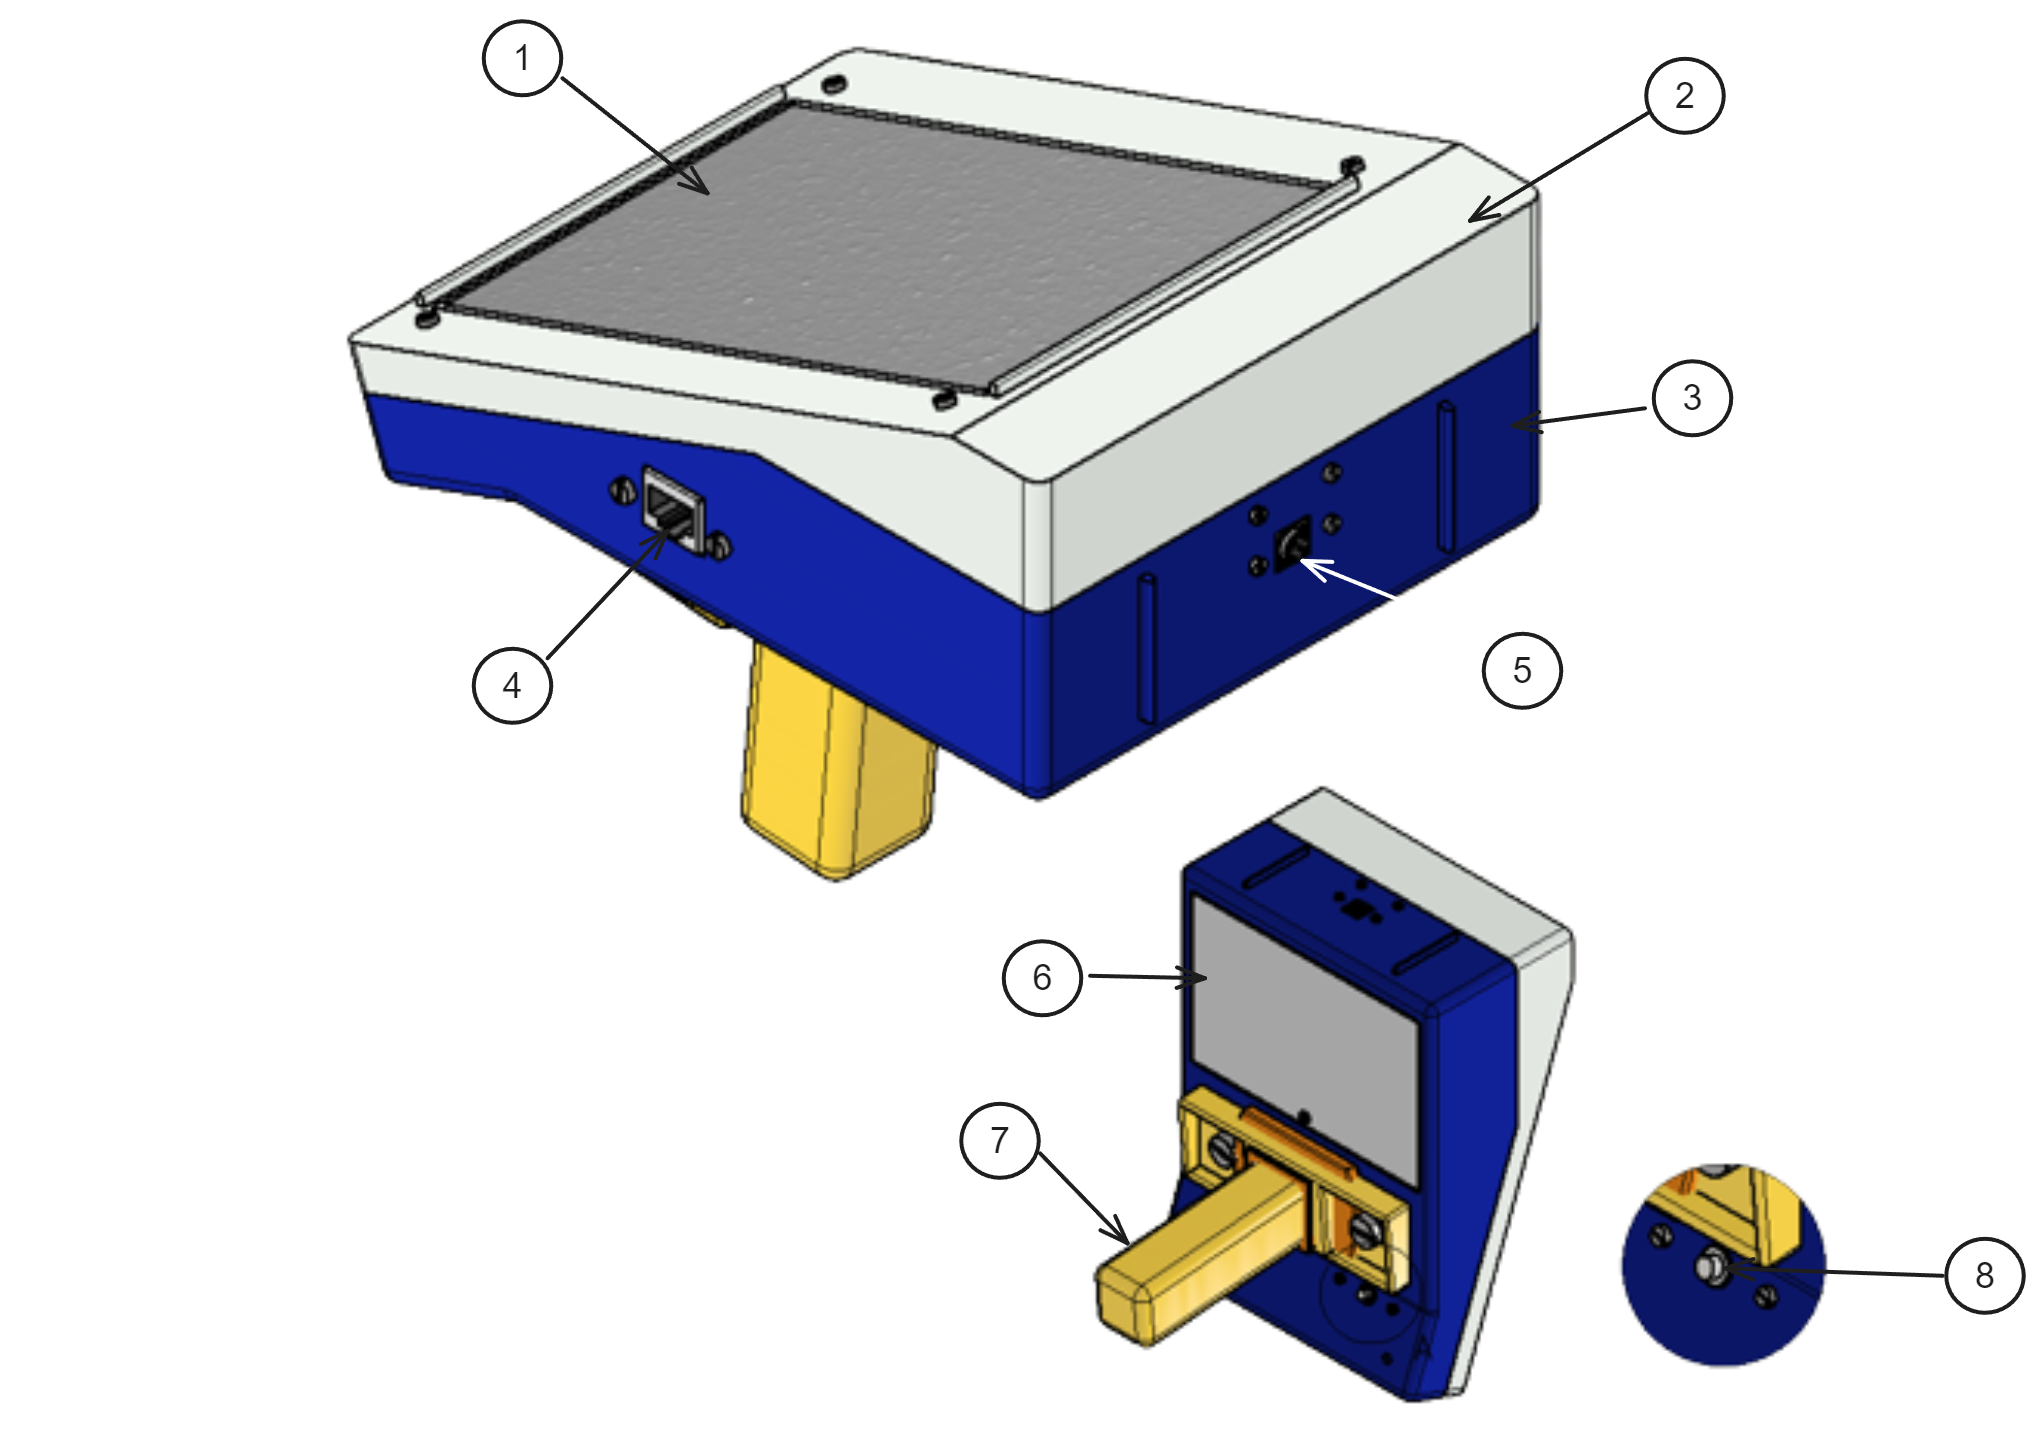
\includegraphics[width=\textwidth]{texs/chapter1/image/111.png}
\end{figure}

\begin{table}
    \centering
    \begin{tabular}{|l|l|}
        \hline
        \textbf{Number} & \textbf{Function} \\ \hline
        1               & Touch Screen      \\ \hline
        2               & Top Cover         \\ \hline
        3               & Main Body         \\ \hline
        4               & LAN Port          \\ \hline
        5               & Camera            \\ \hline
        6               & Battery Cover     \\ \hline
        7               & Handle            \\ \hline
        8               & Switch            \\ \hline
    \end{tabular}
\end{table}

\chapter{Quick Start}

This chapter describes how to use the device. Figure below shows the overall process of using the device.

\begin{figure}[H]
    \centering
    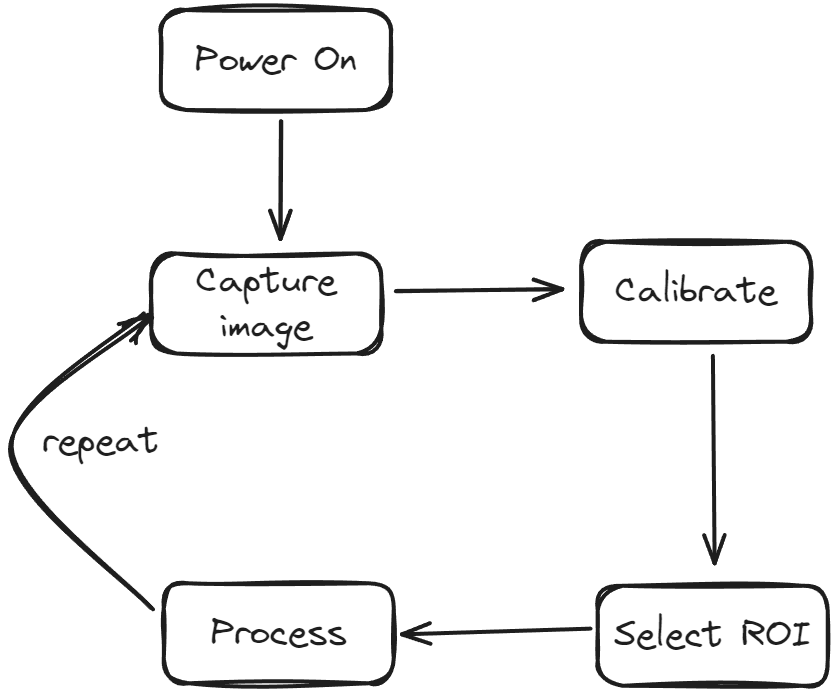
\includegraphics[width=0.8\textwidth]{texs/chapter1/image/overall.png}
\end{figure}

\section{Power On}

\begin{enumerate}
    \item Press the power button to turn on the device.
    \item The device will boot up and the main interface will be displayed.
\end{enumerate}

\section{Capture Image}

\begin{enumerate}
    \item Make sure that you are on the Capture Panel.
    \item Press the Capture button to capture an image.
    \item The captured images will be displayed on the screen.
\end{enumerate}

\section{Calibrate}

\begin{enumerate}
    \item From the Capture Panel, press the Calibrate button to go to the Calibration Panel.
    \item Once you are on the Calibration Panel, press the Start button to start the calibration process.
    \item Depends on the calibration mode, the calibration process will be different.
    \item Once the calibration process is done, press Accept to accept the calibration result.
\end{enumerate}

\section{Select ROI}

\begin{enumerate}
    \item From the Capture Panel, press the ROI button to go to the ROI Selection Panel.
    \item On the ROI Panel, press the Start button to start the ROI selection process.
    \item Within the touchscreen, draw a rectangle to select the region where the object is located.
    \item Once the ROI selection process is done, press Accept to accept the ROI selection result.
\end{enumerate}

\section{Measure}

\begin{enumerate}
    \item From the Capture Panel, press the Measure button to go to the Measurement Panel.
    \item On the Measurement Panel, press the Start button to start the measurement process.
    \item The measurement result will be displayed on the screen.
\end{enumerate}


\chapter{Panel Overview}

This chapter provides information on the available panels and their functions.

Following are the available panels:

\begin{itemize}
    \item Capture Panel
    \item Automatic Lane Calibration Panel
    \item Manual Lane Calibration Panel
    \item Distance Calibration Panel
    \item ROI Panel
    \item Result Panel
    \item Color Calibration Panel
    \item Trim Data Panel
    \item Settings Panel
\end{itemize}

% page break
\pagebreak

\renewcommand\thempfootnote{\arabic{mpfootnote}}


\section{Main Layout}
\label{sec:main-layout}

This section provides information on the main layout of the device. Most of the available panels have the same layout.

\begin{figure}[H]
    \centering
    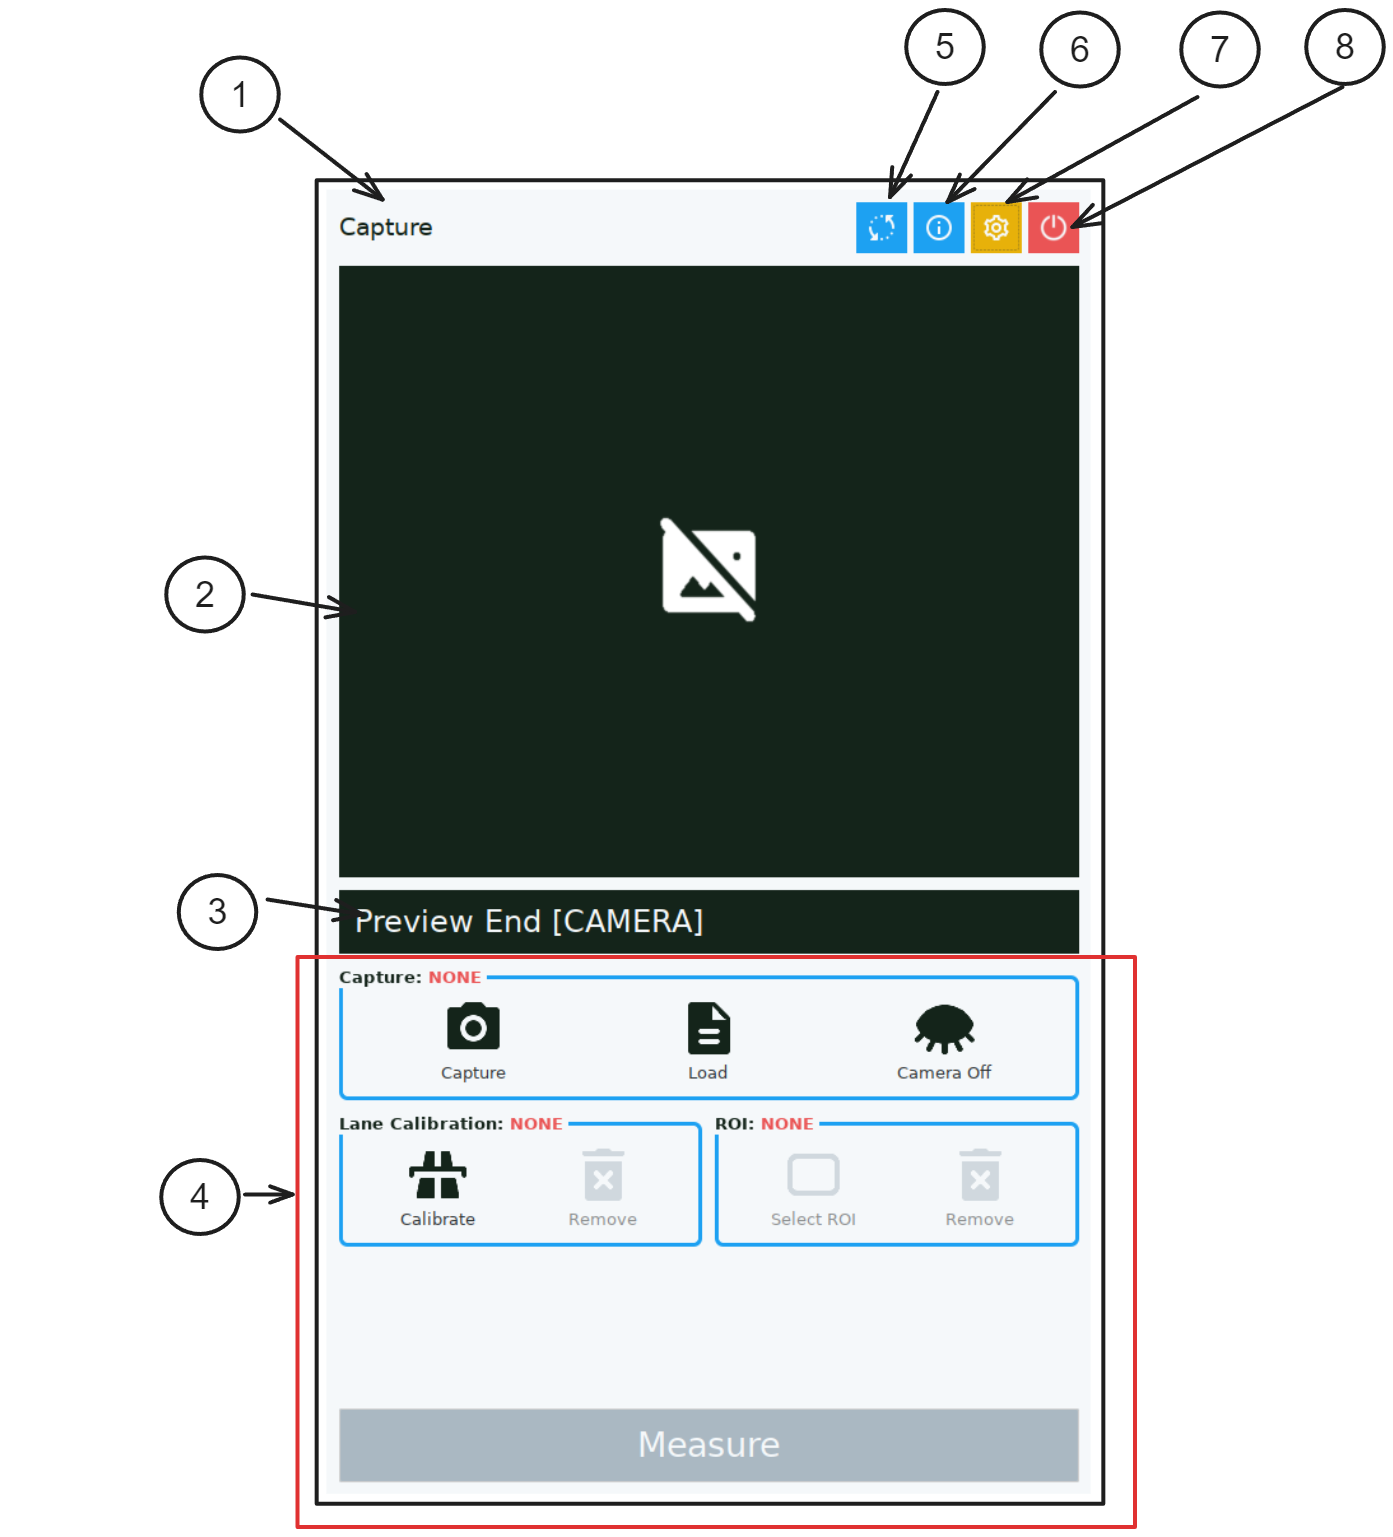
\includegraphics[width=0.5\textwidth]{texs/chapter1/image/p9.png}
\end{figure}

\begin{table}[!ht]
    \centering
    \begin{minipage}{\textwidth} % <--- new
        \begin{tabular}{p{0.05\linewidth} | p{0.3\linewidth} | p{0.5\linewidth}}
            \hline
            \textbf{No.} & \textbf{Name}                                                                                       & \textbf{Function}                                 \\ \hline
            1            & Title                                                                                               & Show current panel                                \\ \hline
            2            & Image Panel                                                                                         & Show Image                                        \\ \hline
            3            & Status Panel                                                                                        & Display status of application                     \\ \hline
            4            & Button Panel                                                                                        & Contains all buttons for processes and navigation \\ \hline
            5            & Switch Mode Button\footnote{This button only appear on \hyperref[sec:capture-panel]{Capture Panel}} & Switch between DISTANCE and LANE mode             \\ \hline
            6            & Info Button                                                                                         & Show Info                                         \\ \hline
            7            & Settings Button                                                                                     & Switch to Settings Panel                          \\ \hline
            8            & Exit Button                                                                                         & Exit the Application                              \\ \hline
        \end{tabular}
    \end{minipage} % <--- new
\end{table}

\pagebreak
\section{Capture Panel}
\label{sec:capture-panel}

This section provides information on the Capture Panel. This Panel will handle the image capturing process. Additionally this panel also provides the ability to save and load captured data.

\begin{figure}[H]
    \centering
    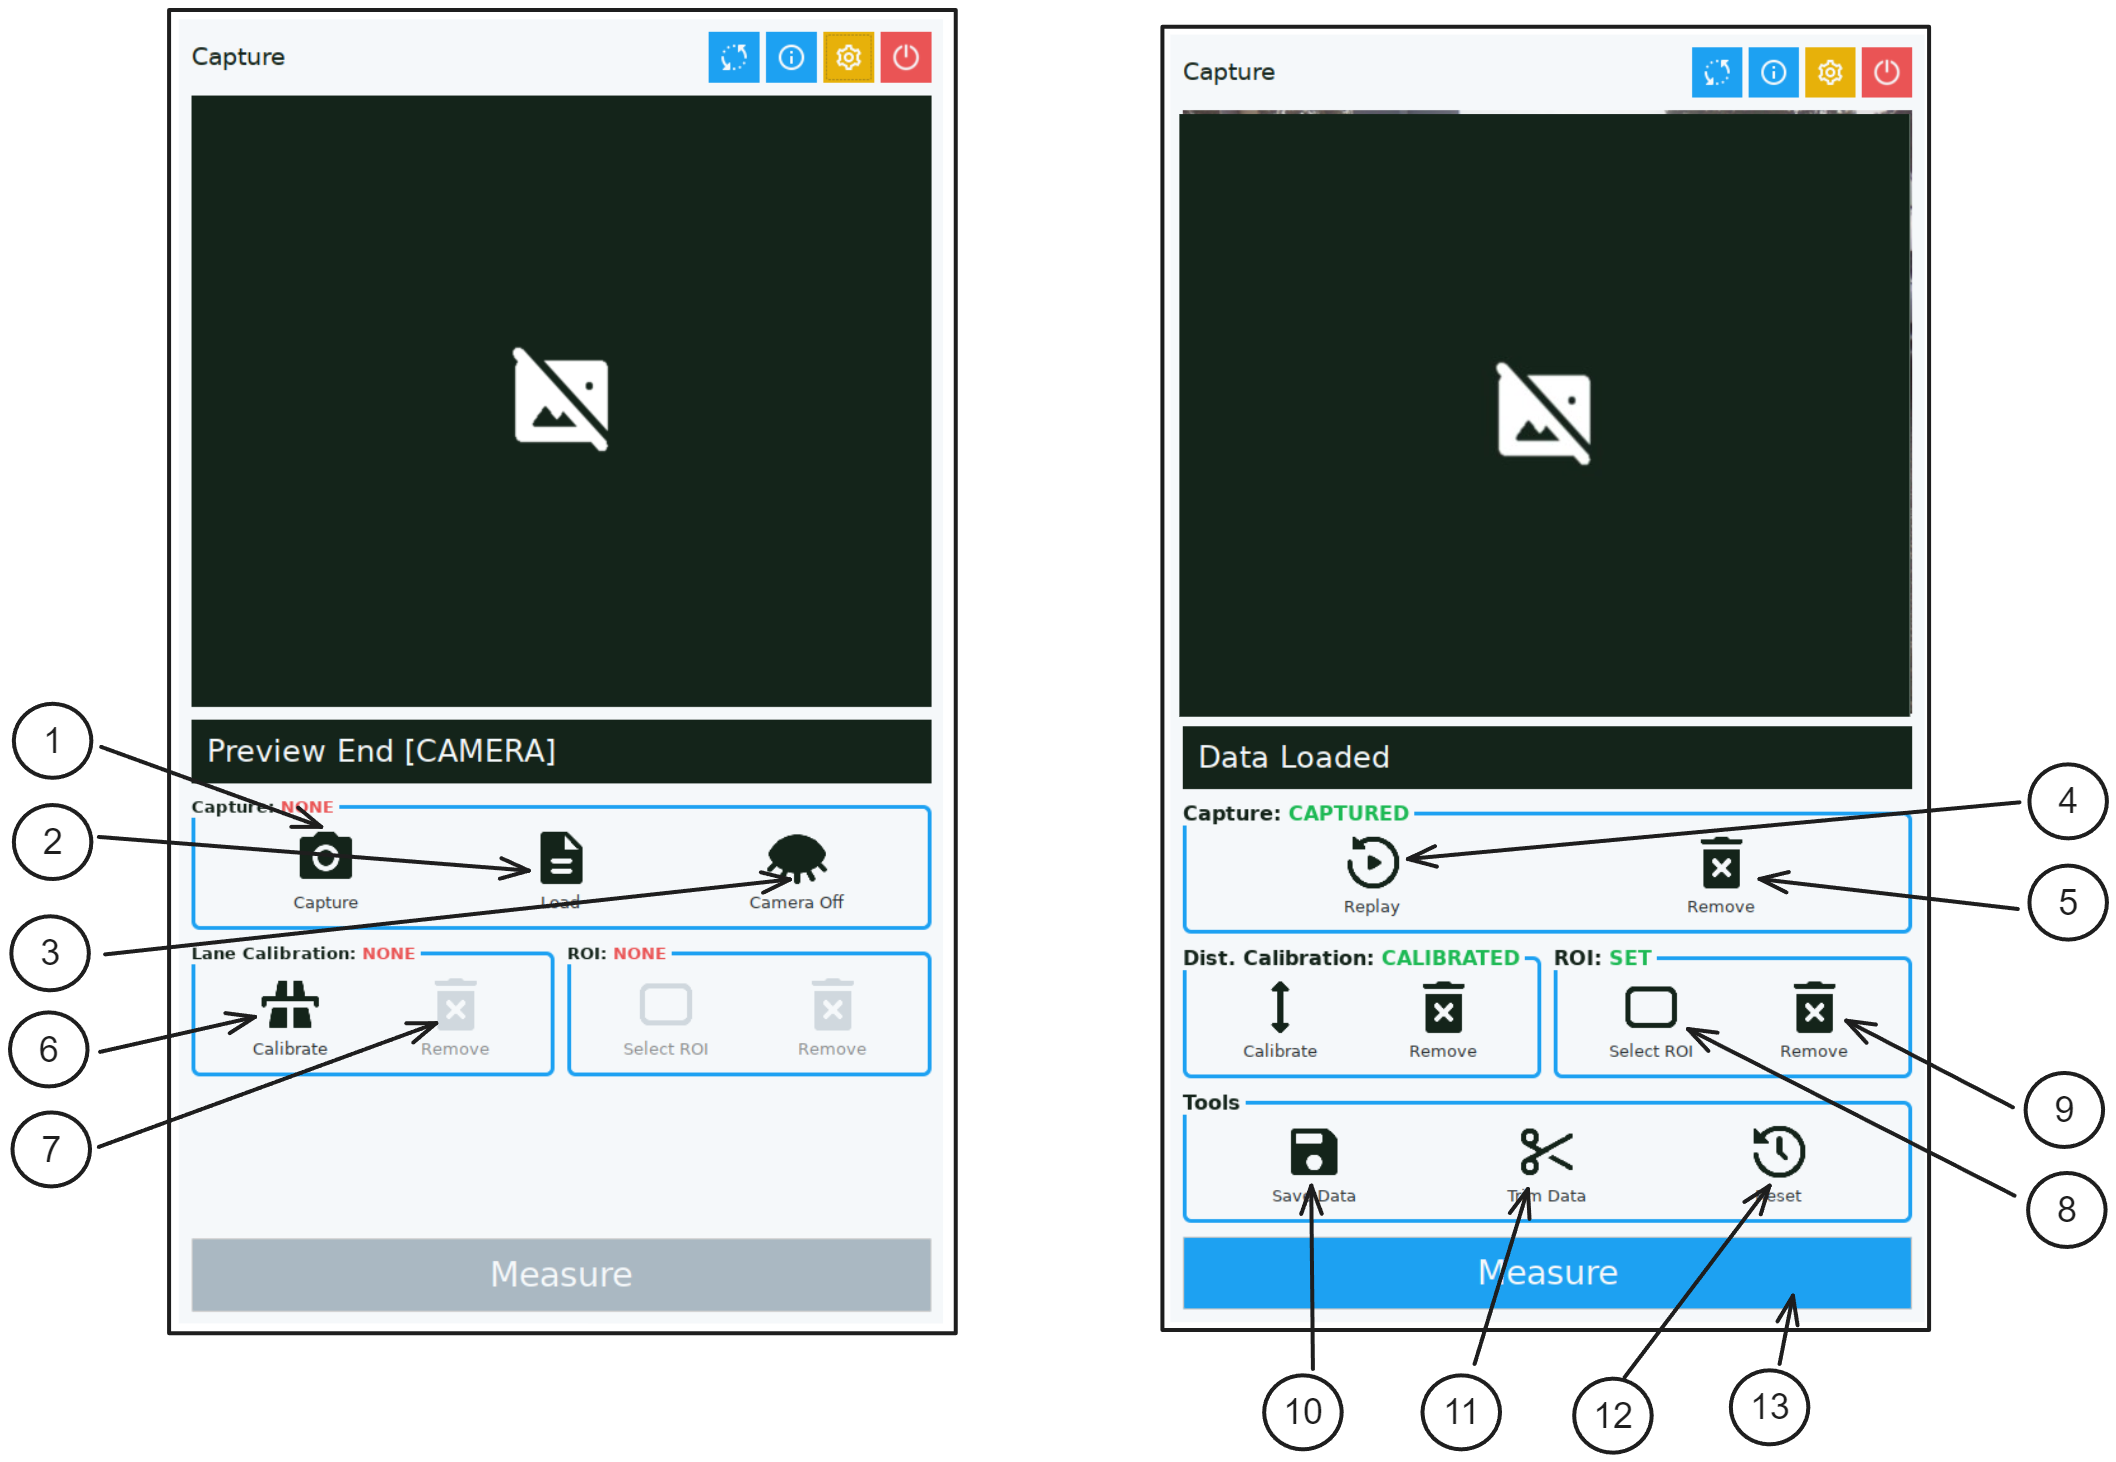
\includegraphics[width=0.65\textwidth]{texs/chapter1/image/p1.png}
\end{figure}

\begin{table}[!ht]
    \centering
    \begin{tabular}{p{0.05\linewidth} | p{0.5\linewidth}}
        \hline
        \textbf{No} & \textbf{Function}                \\ \hline
        1           & Capture Image                    \\ \hline
        2           & Load Saved data                  \\ \hline
        3           & Toggle Camera On / Off (Preview) \\ \hline
        4           & Replay Captured Data             \\ \hline
        5           & Clear/Remove Captured Data       \\ \hline
        6           & Change to Calibration Panel      \\ \hline
        7           & Remove Calibration Data          \\ \hline
        8           & Change To Roi Panel              \\ \hline
        9           & Remove Roi Data                  \\ \hline
        10          & Save Captured  Data              \\ \hline
        11          & Trim Captured Data               \\ \hline
        12          & Reset Session (Remove All Data)  \\ \hline
        13          & Change To Result Panel           \\ \hline
    \end{tabular}
\end{table}

\subsection{Instructions}

\subsubsection{Capture Image}
To capture image press the Capture button (\textbf{1}). The image will be captured and displayed in the panel. The image will also be saved in the program's memory.

\subsubsection{Load Saved Data}
To load saved data press the Load button (\textbf{2}). A file dialog will appear. Select the file you want to load. The file will be loaded and displayed in the panel. The file will also be saved in the program's memory.

\subsubsection{Toggle Camera On / Off (Preview)}
To toggle the camera on or off press the Camera button (\textbf{3}). The camera will be turned on or off. If the camera is on, the image will be displayed in the panel.

\subsubsection{Replay Captured Data}
To replay the captured data press the Replay button (\textbf{4}). Make sure that the data is loaded. The data will be replayed in the panel.

\subsubsection{Clear/Remove Captured Data}
To clear/remove the captured data press the Clear button (\textbf{5}). The data will be cleared/removed from the program's memory.

\subsubsection{Change to Calibration Panel}
To change to the Calibration Panel press the Calibration button (\textbf{6}). The Calibration Panel will be displayed. Refer \hyperref[sec:auto-lane-calibration-panel]{Automatic Lane Calibration Panel} and \hyperref[sec:distance-calibration-panel]{Distance Calibration Panel} for more information.

\subsubsection{Remove Calibration Data}
To remove the calibration data press the Remove Calibration button (\textbf{7}). The calibration data will be removed from the program's memory. If ROI data is present, it will also be removed.

\subsubsection{Change To Roi Panel}
To change to the Roi Panel press the Roi button (\textbf{8}). The Roi Panel will be displayed. Refer \hyperref[sec:roi-panel]{Roi Panel} for more information.

\subsubsection{Remove Roi Data}
To remove the Roi data press the Remove Roi button (\textbf{9}). The Roi data will be removed from the program's memory.

\subsubsection{Save Captured  Data}
To save the captured data press the Save button (\textbf{10}). A file dialog will appear. If you press accept, the data will be saved to the file you selected.

\subsubsection{Trim Captured Data}
To trim the captured data press the Trim button (\textbf{11}). A dialog will appear. The TrimDataPanel will be displayed. Refer \hyperref[sec:trim-data-panel]{Trim Data Panel} for more information.

\subsubsection{Reset Session (Remove All Data)}
To reset the session press the Reset button (\textbf{12}). All the data will be removed from the program's memory.

\subsubsection{Change To Result Panel}
To change to the Result Panel press the Result button (\textbf{13}). The Result Panel will be displayed. Refer \hyperref[sec:result-panel]{Result Panel} for more information.

\pagebreak
\section{Automatic Lane Calibration Panel}
\label{sec:auto-lane-calibration-panel}

The Calibration Panel is where you can perform automatic lane calibration. This calibration type is done with the custom mat.\footnote{Please make sure that you adjust the object size in the Settings Panel. Go to settings panel by pressing the Settings button. Locate the \textbf{Object Width} variable and adjust it to the width of the mat (420 mm).}\footnote{To perform this calibration type, make sure the application is in \textbf{LANE MEASUREMENT MODE} by pressing the \textbf{Toggle Mode} button. Refer to \hyperref[sec:main-layout]{Main Layout} for more information.}

\begin{figure}[H]
    \centering
    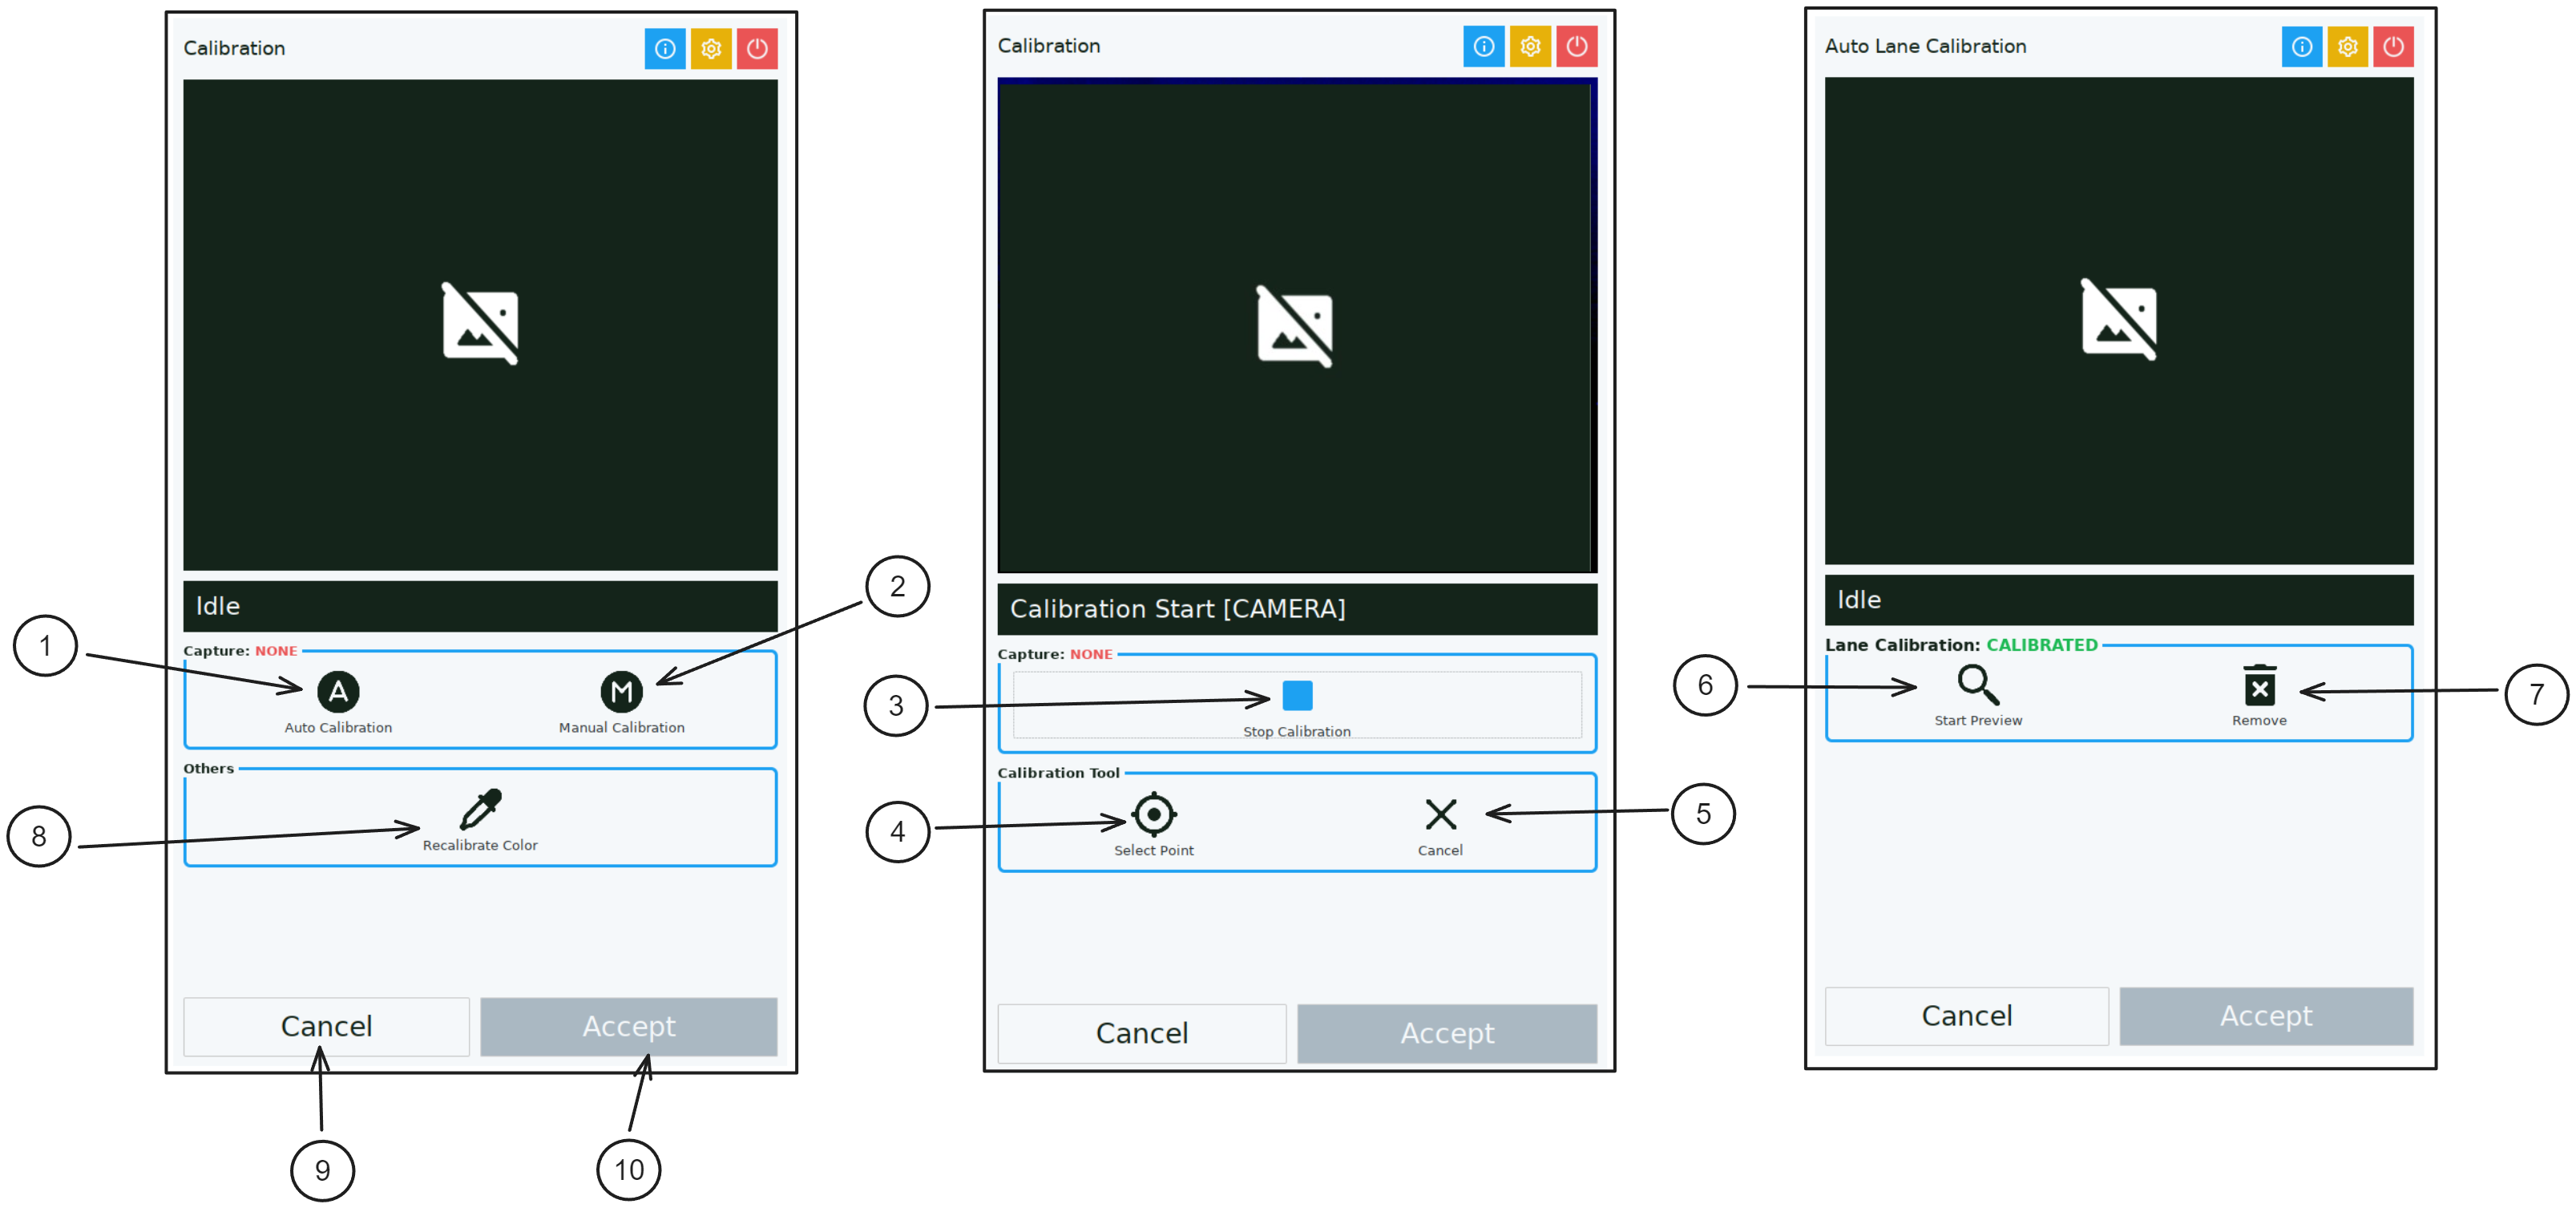
\includegraphics[width=\textwidth]{texs/chapter1/image/p2.png}
\end{figure}

\begin{table}[!ht]
    \centering
    \begin{tabular}{p{0.05\linewidth} | p{0.5\linewidth}}
        \hline
        \textbf{No.} & \textbf{Function}                       \\ \hline
        1            & Start Automatic Lane Calibration        \\ \hline
        2            & Change To Manual Lane Calibration Panel \\ \hline
        3            & Stop Calibration                        \\ \hline
        4            & Select Point                            \\ \hline
        5            & Cancel / Remove Calibration             \\ \hline
        6            & Start Preview / Show Calibrated Data    \\ \hline
        7            & Remove Calibrated Data                  \\ \hline
        8            & Change To Color Calibration Panel       \\ \hline
        9            & Cancel Calibration                      \\ \hline
        10           & Accept Calibration                      \\ \hline
    \end{tabular}
\end{table}

\subsection{Instructions}

\subsubsection{Performing Calibration}

To perform automatic lane calibration, press the Start Calibration button (\textbf{1}). The program will start the calibration process. The program will display the image in the panel. Begin with selecting point by pressing the Select Point button (\textbf{4}). After clicking the point, select on the Image Panel, the position where the mat is located. The program will automatically detect line and display it in the panel. If the line is not detected, try to select another point. If the line is detected, press the Accept Calibration button (\textbf{10}). The program will save the calibration data in the program's memory.

\subsubsection{Start Preview / Show Calibrated Data}

To start preview or show calibrated data press the Preview button (\textbf{6}). The program will display the image in the panel. If the calibration data is present, the program will display the calibrated data in the panel.

\subsubsection{Change To Manual Lane Calibration Panel}

To change to the Manual Lane Calibration Panel press the Manual Calibration button (\textbf{2}). The Manual Lane Calibration Panel will be displayed. Refer \hyperref[sec:manual-lane-calibration-panel]{Manual Lane Calibration Panel} for more information.

\subsubsection{Change To Color Calibration Panel}

To change to the Color Calibration Panel press the Color Calibration button (\textbf{8}). The Color Calibration Panel will be displayed. Refer \hyperref[sec:color-calibration-panel]{Color Calibration Panel} for more information.

\pagebreak
\section{Manual Lane Calibration Panel}
\label{sec:manual-lane-calibration-panel}

The Manual Lane Calibration Panel is where you can perform manual lane calibration.\footnote{Please make sure that you adjust the object size in the Settings Panel. Go to settings panel by pressing the Settings button. Locate the \textbf{Object Width} variable and adjust it to the width of the mat (420 mm) or width of road (3500 mm)}\footnote{To perform this calibration type, make sure the application is in \textbf{LANE MEASUREMENT MODE} by pressing the \textbf{Toggle Mode} button. Refer to \hyperref[sec:main-layout]{Main Layout} for more information.}

\begin{figure}[H]
    \centering
    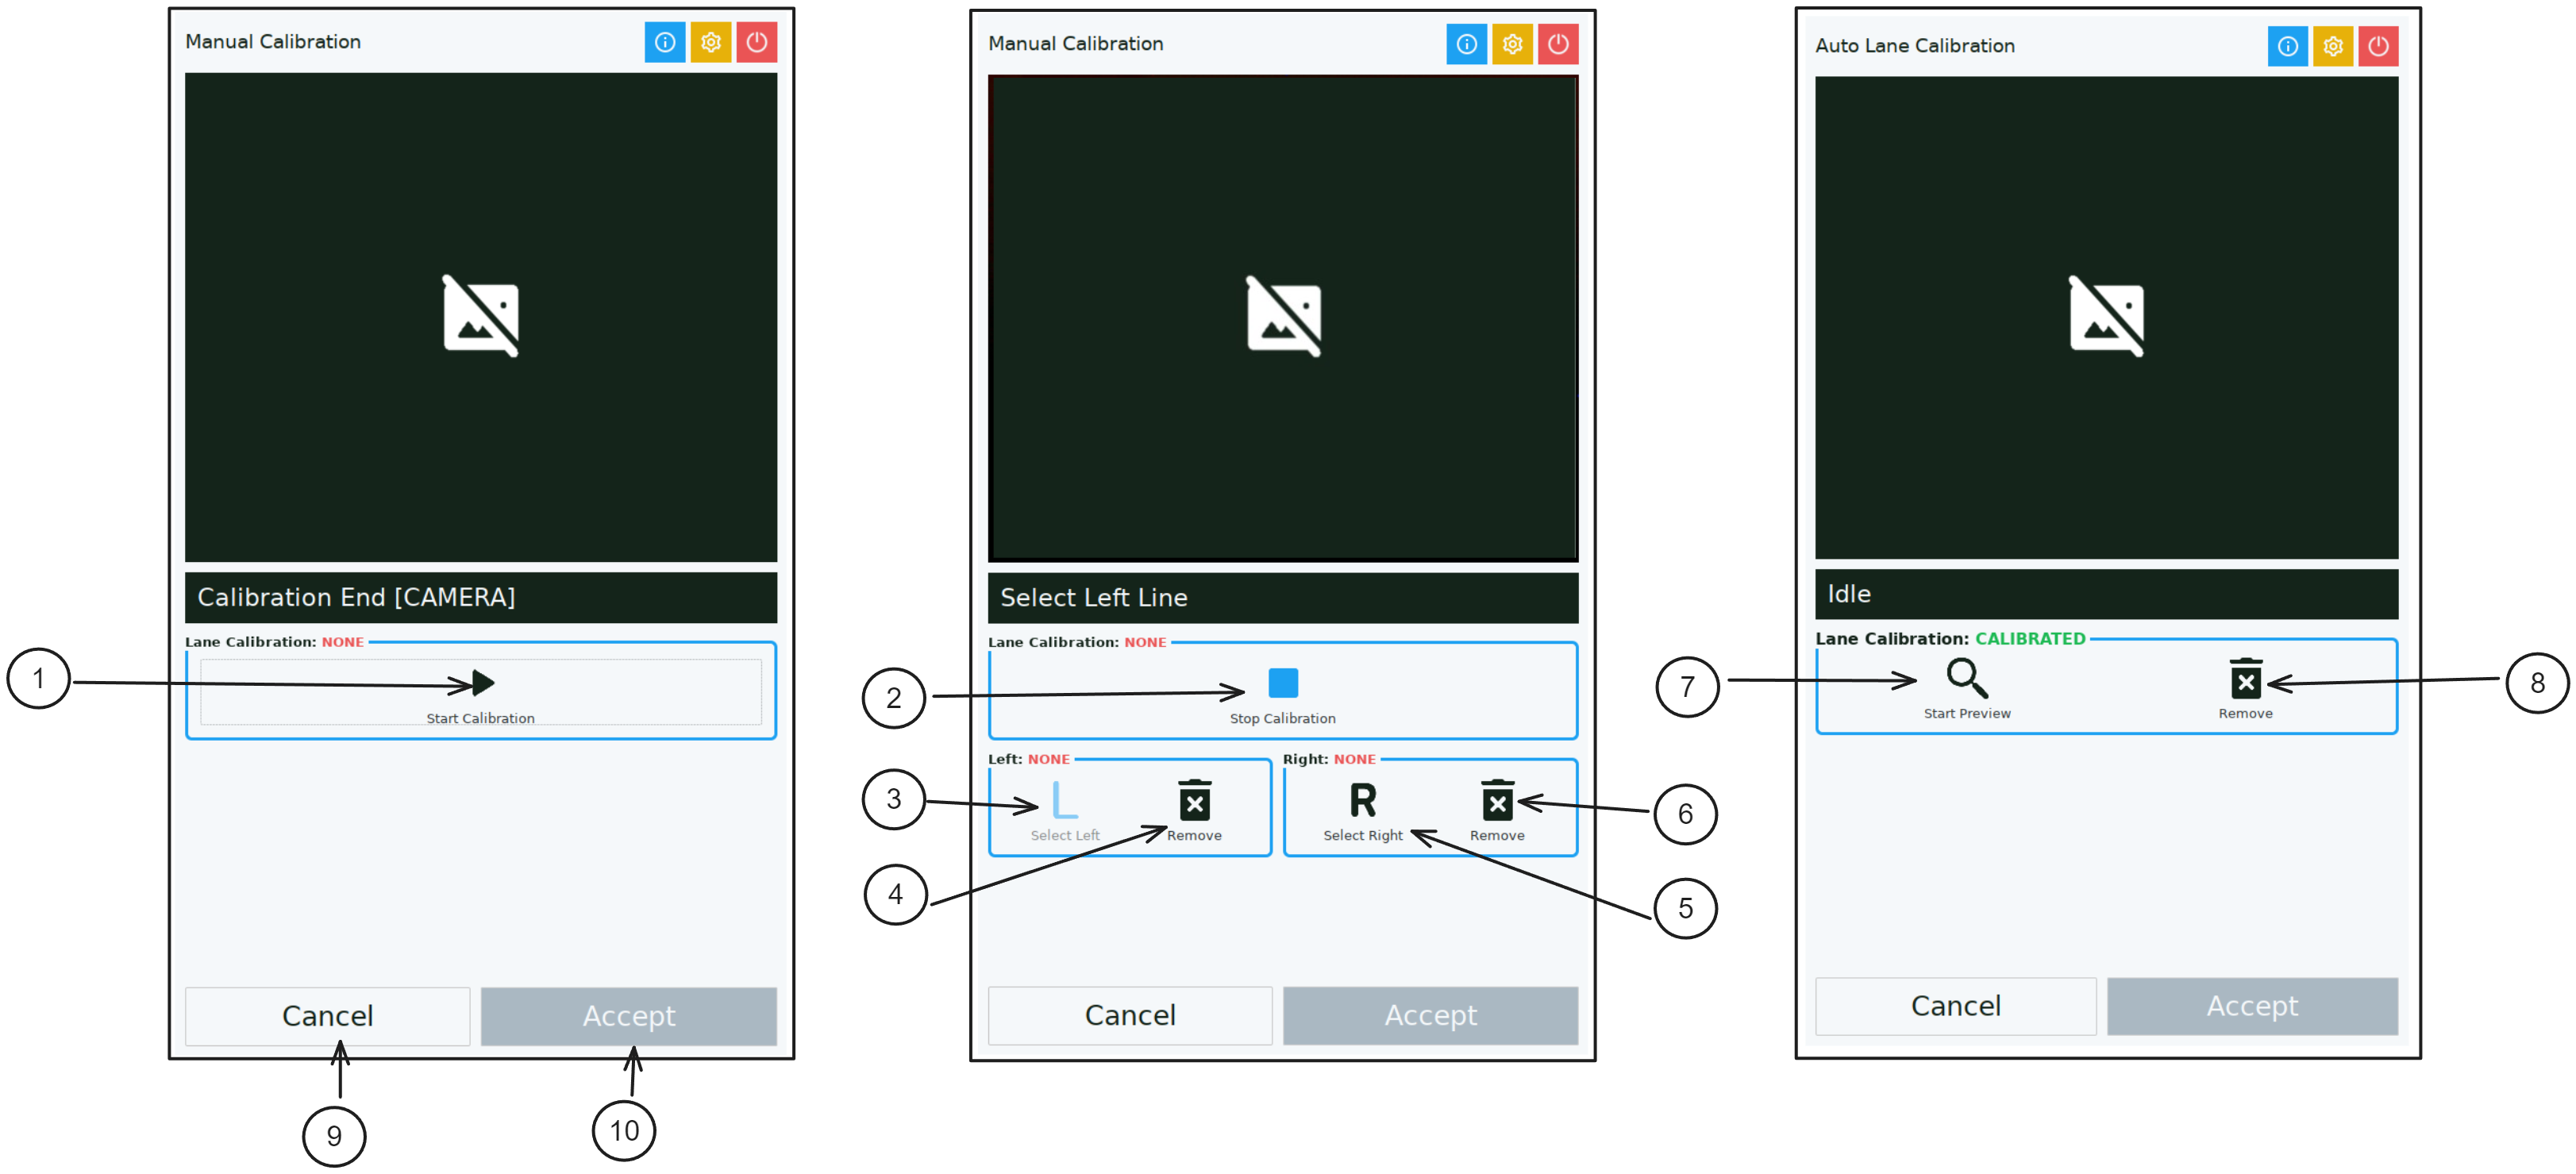
\includegraphics[width=\textwidth]{texs/chapter1/image/p3.png}
\end{figure}

\begin{table}[!ht]
    \centering
    \begin{tabular}{p{0.05\linewidth} | p{0.5\linewidth}}
        \hline
        \textbf{No.} & \textbf{Function}                    \\ \hline
        1            & Start Manual Lane Calibration        \\ \hline
        2            & Stop Calibration                     \\ \hline
        3            & Select Left Line                     \\ \hline
        4            & Remove Selected Left Line            \\ \hline
        5            & Select Right Line                    \\ \hline
        6            & Remove Selected Right Line           \\ \hline
        7            & Start Preview / Show Calibrated Data \\ \hline
        8            & Remove Calibrated Data               \\ \hline
        9            & Cancel Calibration                   \\ \hline
        10           & Accept Calibration                   \\ \hline
    \end{tabular}
\end{table}

\subsection{Instructions}

\subsubsection{Performing Calibration}

To perform manual lane calibration, press the Start Calibration button (\textbf{1}). The program will start the calibration process. The program will display the image in the panel. Begin with selecting the left line by pressing the Select Left Line button (\textbf{3}). Line selection is done via point and drag method. Place the finger on the Image Panel where the starting point of the object is located. Adjust the position by dragging the finger. Repeat the process for the right line by pressing the Select Right Line button (\textbf{5}). After selecting both lines, press the Accept Calibration button (\textbf{10}). The program will save the calibration data in the program's memory.

\subsubsection{Start Preview / Show Calibrated Data}

To start preview or show calibrated data press the Preview button (\textbf{7}). The program will display the image in the panel. If the calibration data is present, the program will display the calibrated data in the panel.

\pagebreak
\section{Distance Calibration Panel}
\label{sec:distance-calibration-panel}

The Distance Calibration Panel is where you can perform distance calibration. This calibration is done with an object of known height.\footnote{Please make sure that you adjust the object size in the Settings Panel. Go to settings panel by pressing the Settings button. Locate the \textbf{Object Height} variable and adjust it to the height of the object.}\footnote{To perform this calibration type, make sure the application is in \textbf{DISTANCE MEASUREMENT MODE} by pressing the \textbf{Toggle Mode} button. Refer to \hyperref[sec:main-layout]{Main Layout} for more information.}

\begin{figure}[H]
    \centering
    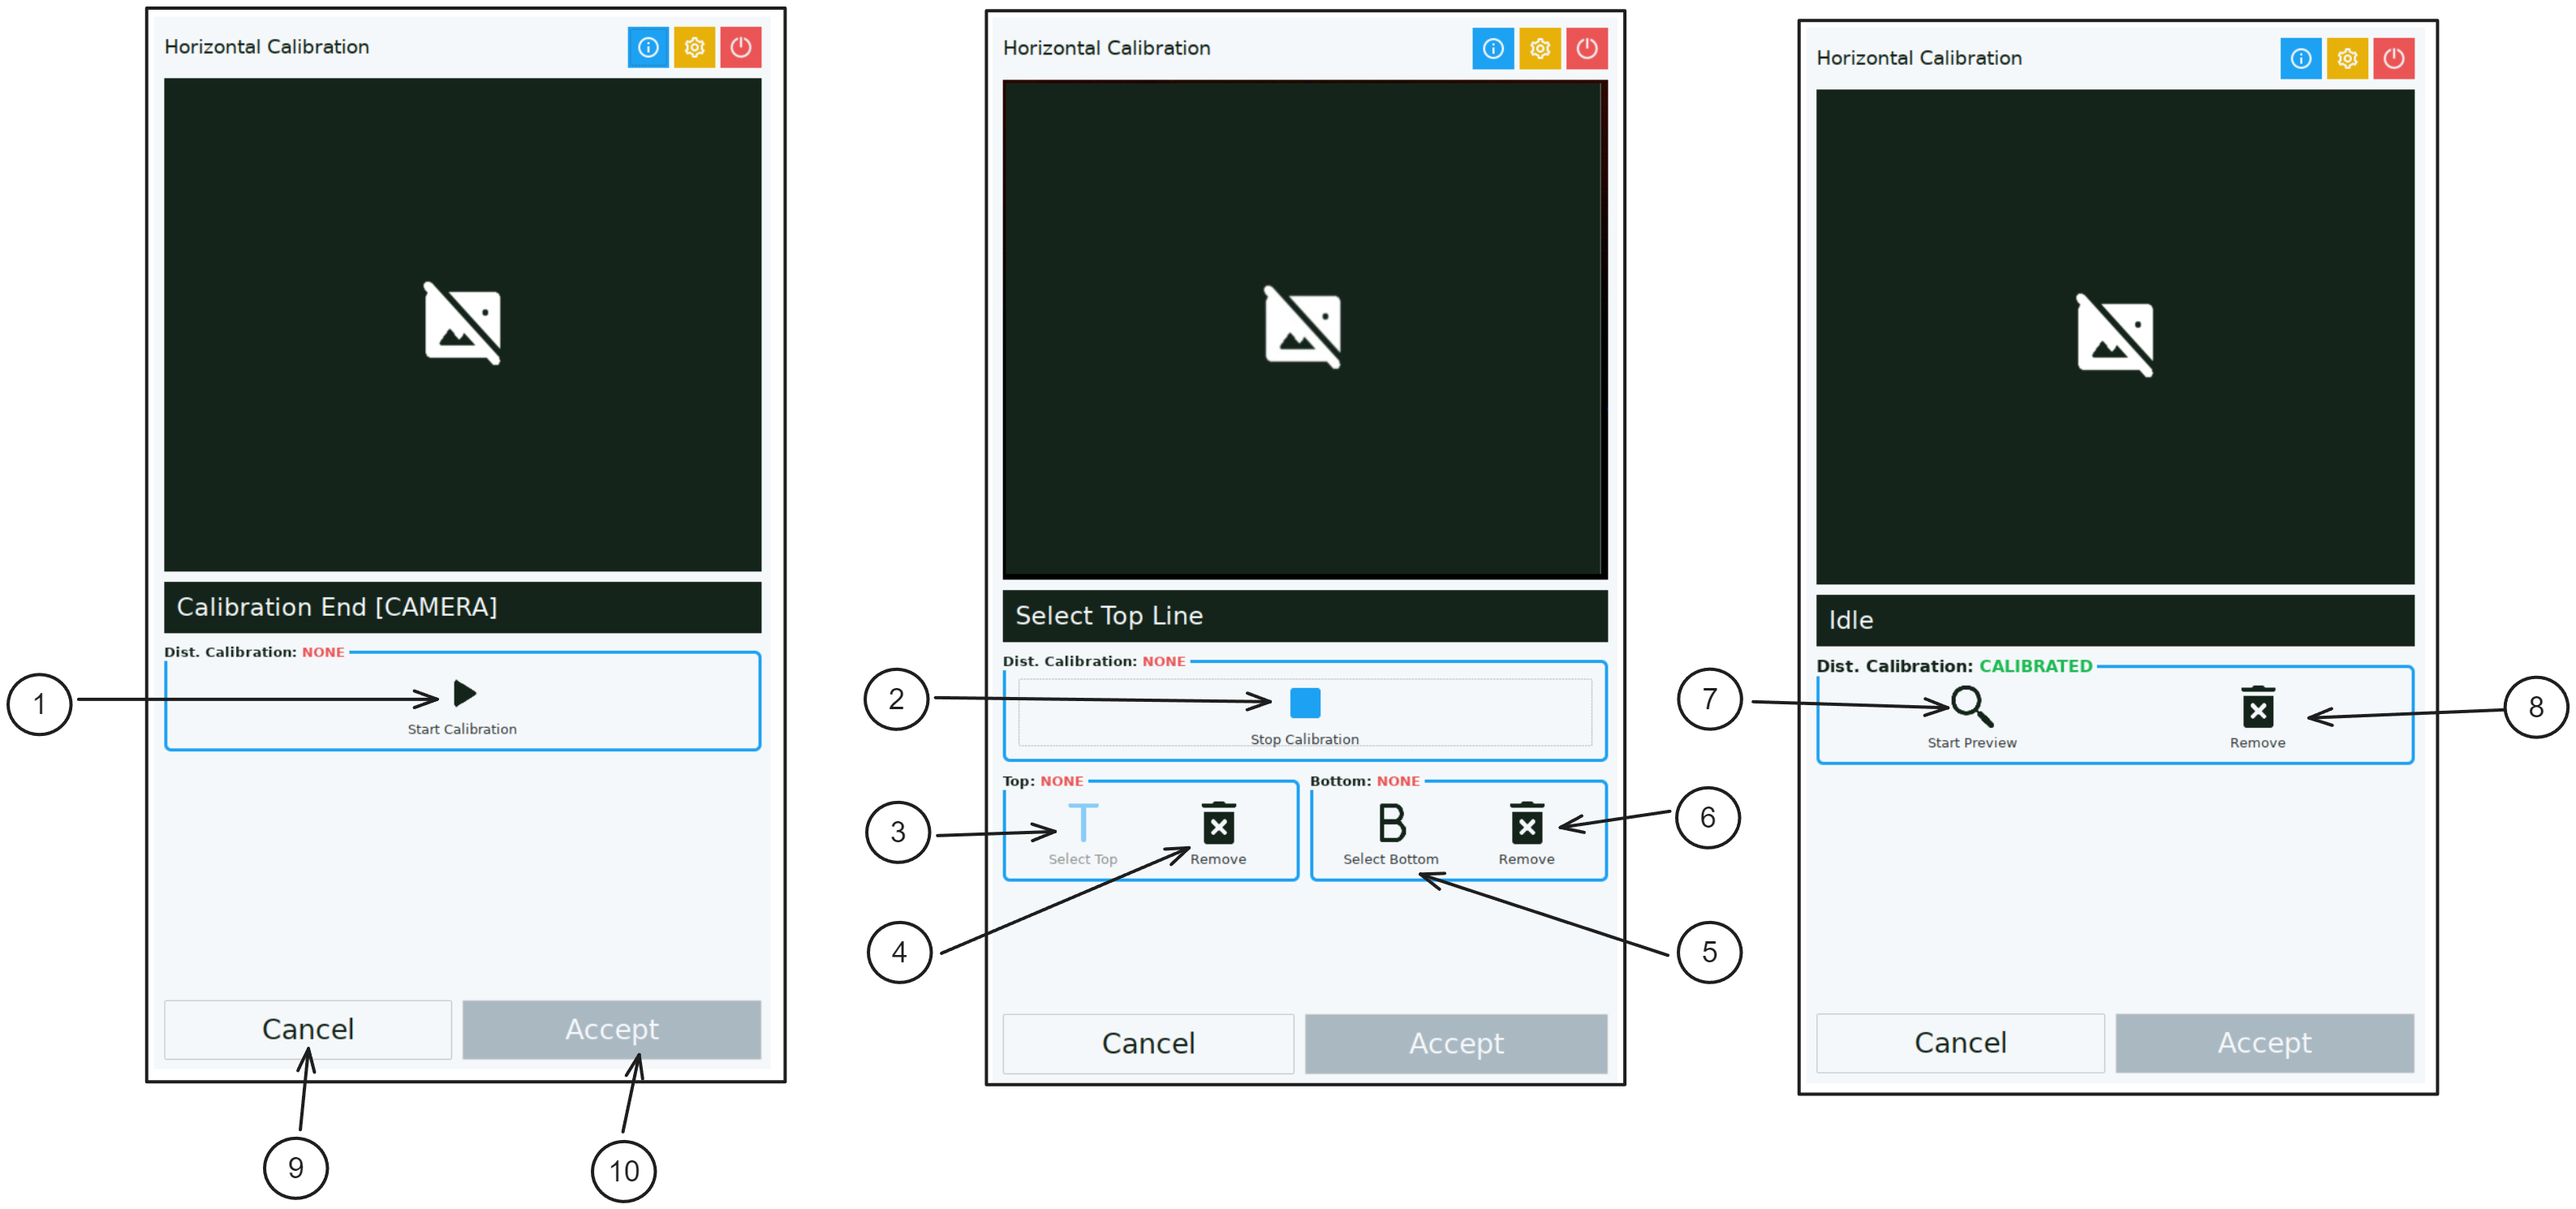
\includegraphics[width=\textwidth]{texs/chapter1/image/p4.png}
\end{figure}

\begin{table}[!ht]
    \centering
    \begin{tabular}{p{0.05\linewidth} | p{0.5\linewidth}}
        \hline
        \textbf{No.} & \textbf{Function}                    \\ \hline
        1            & Start Distance Calibration           \\ \hline
        2            & Stop Calibration                     \\ \hline
        3            & Select Top Line                      \\ \hline
        4            & Remove Selected Top Line             \\ \hline
        5            & Select Bottom Line                   \\ \hline
        6            & Remove Selected Bottom Line          \\ \hline
        7            & Start Preview / Show Calibrated Data \\ \hline
        8            & Remove Calibrated Data               \\ \hline
        9            & Cancel Calibration                   \\ \hline
        10           & Accept Calibration                   \\ \hline
    \end{tabular}
\end{table}

\subsection{Instructions}

\subsubsection{Performing Calibration}

To perform distance calibration, press the Start Calibration button (\textbf{1}). The program will start the calibration process. The program will display the image in the panel. Begin with selecting the top line by pressing the Select Top Line button (\textbf{3}). Line selection is done via point and drag method. Place the finger on the Image Panel where the starting point of the object is located. Adjust the position by dragging the finger. Repeat the process for the bottom line by pressing the Select Bottom Line button (\textbf{5}). After selecting both lines, press the Accept Calibration button (\textbf{10}). The program will save the calibration data in the program's memory.

\subsubsection{Start Preview / Show Calibrated Data}

To start preview or show calibrated data press the Preview button (\textbf{7}). The program will display the image in the panel. If the calibration data is present, the program will display the calibrated data in the panel.

\pagebreak
\section{Roi Panel}
\label{sec:roi-panel}

The Roi Panel is where you can perform region of interest (ROI) selection.

\begin{figure}[H]
    \centering
    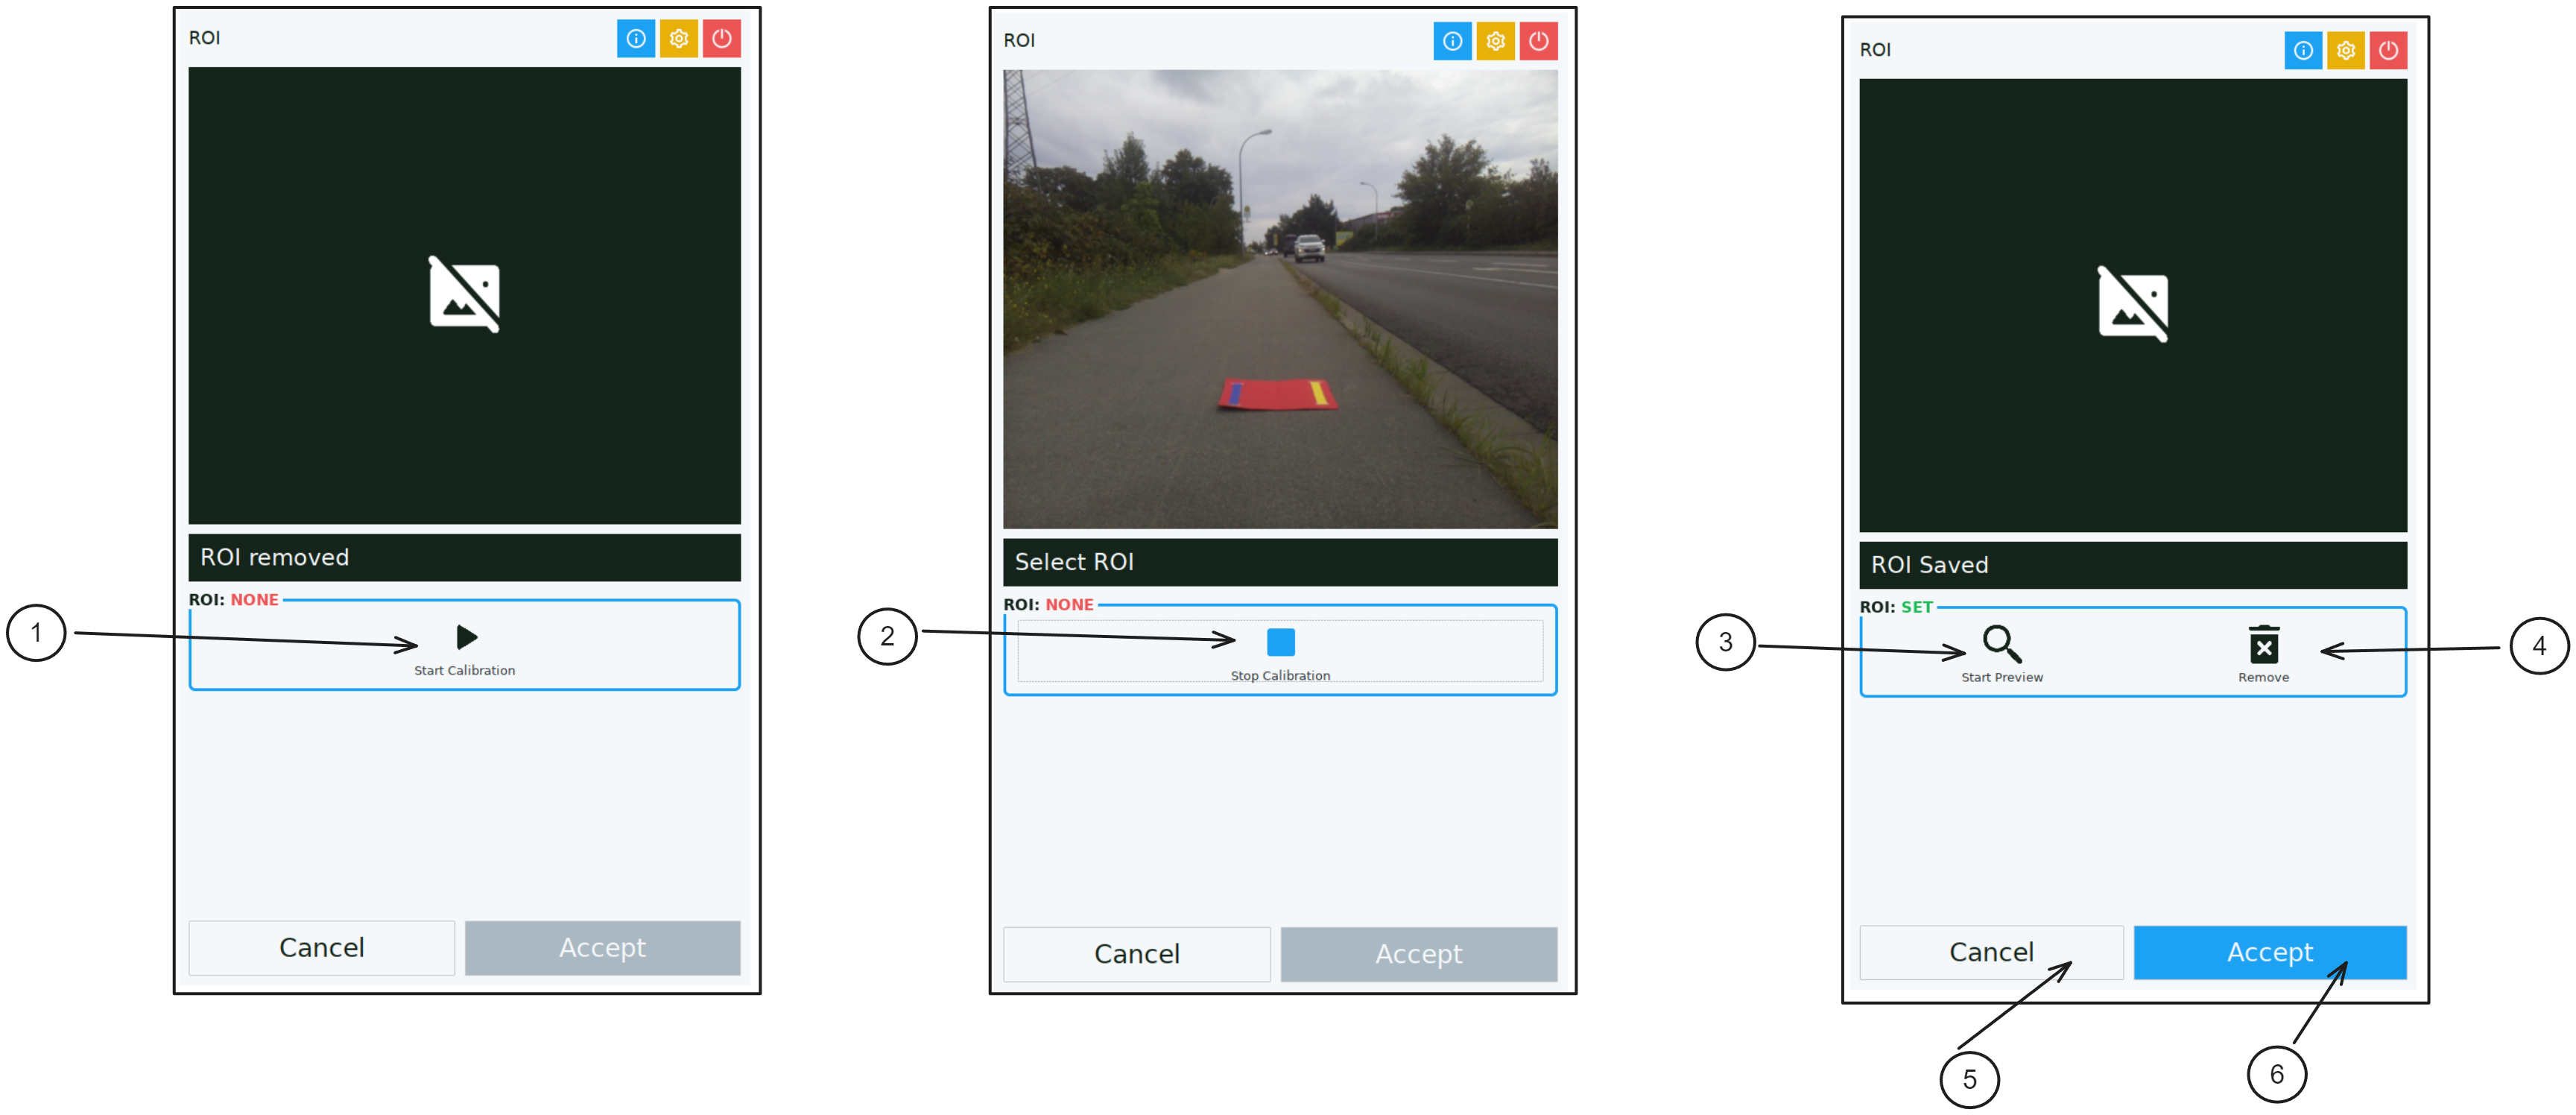
\includegraphics[width=\textwidth]{texs/chapter1/image/p8.png}
\end{figure}

\begin{table}[!ht]
    \centering
    \begin{tabular}{p{0.05\linewidth} | p{0.5\linewidth}}
        \hline
        \textbf{No.} & \textbf{Function} \\ \hline
        1            & Start Roi         \\ \hline
        2            & Stop Roi          \\ \hline
        3            & Start Preview     \\ \hline
        4            & Remove Roi        \\ \hline
        5            & Cancel            \\ \hline
        6            & Accept            \\ \hline
    \end{tabular}
\end{table}

\subsection{Instructions}

\subsubsection{Performing ROI Selection}

To perform ROI selection, press the Start Roi button (\textbf{1}). The program will start the ROI selection process. The program will display the image in the panel. Begin with selecting the top left point by pressing the Select Top Left Point button (\textbf{3}). Point selection is done via point and drag method. Place the finger on the Image Panel where the starting point of the ROI is located. Drag the finger to the end of the ROI. Press the Accept button (\textbf{6}) to accept the ROI. The program will save the ROI data in the program's memory.

\subsubsection{Start Preview}

To start preview the ROI press the Preview button (\textbf{3}). The program will display the image in the panel. If the ROI data is present, the program will display the ROI in the panel.

\pagebreak
\section{Result Panel}
\label{sec:result-panel}

The Result Panel is where you can perform data processing and view the result of the measurement.

\begin{figure}[H]
    \centering
    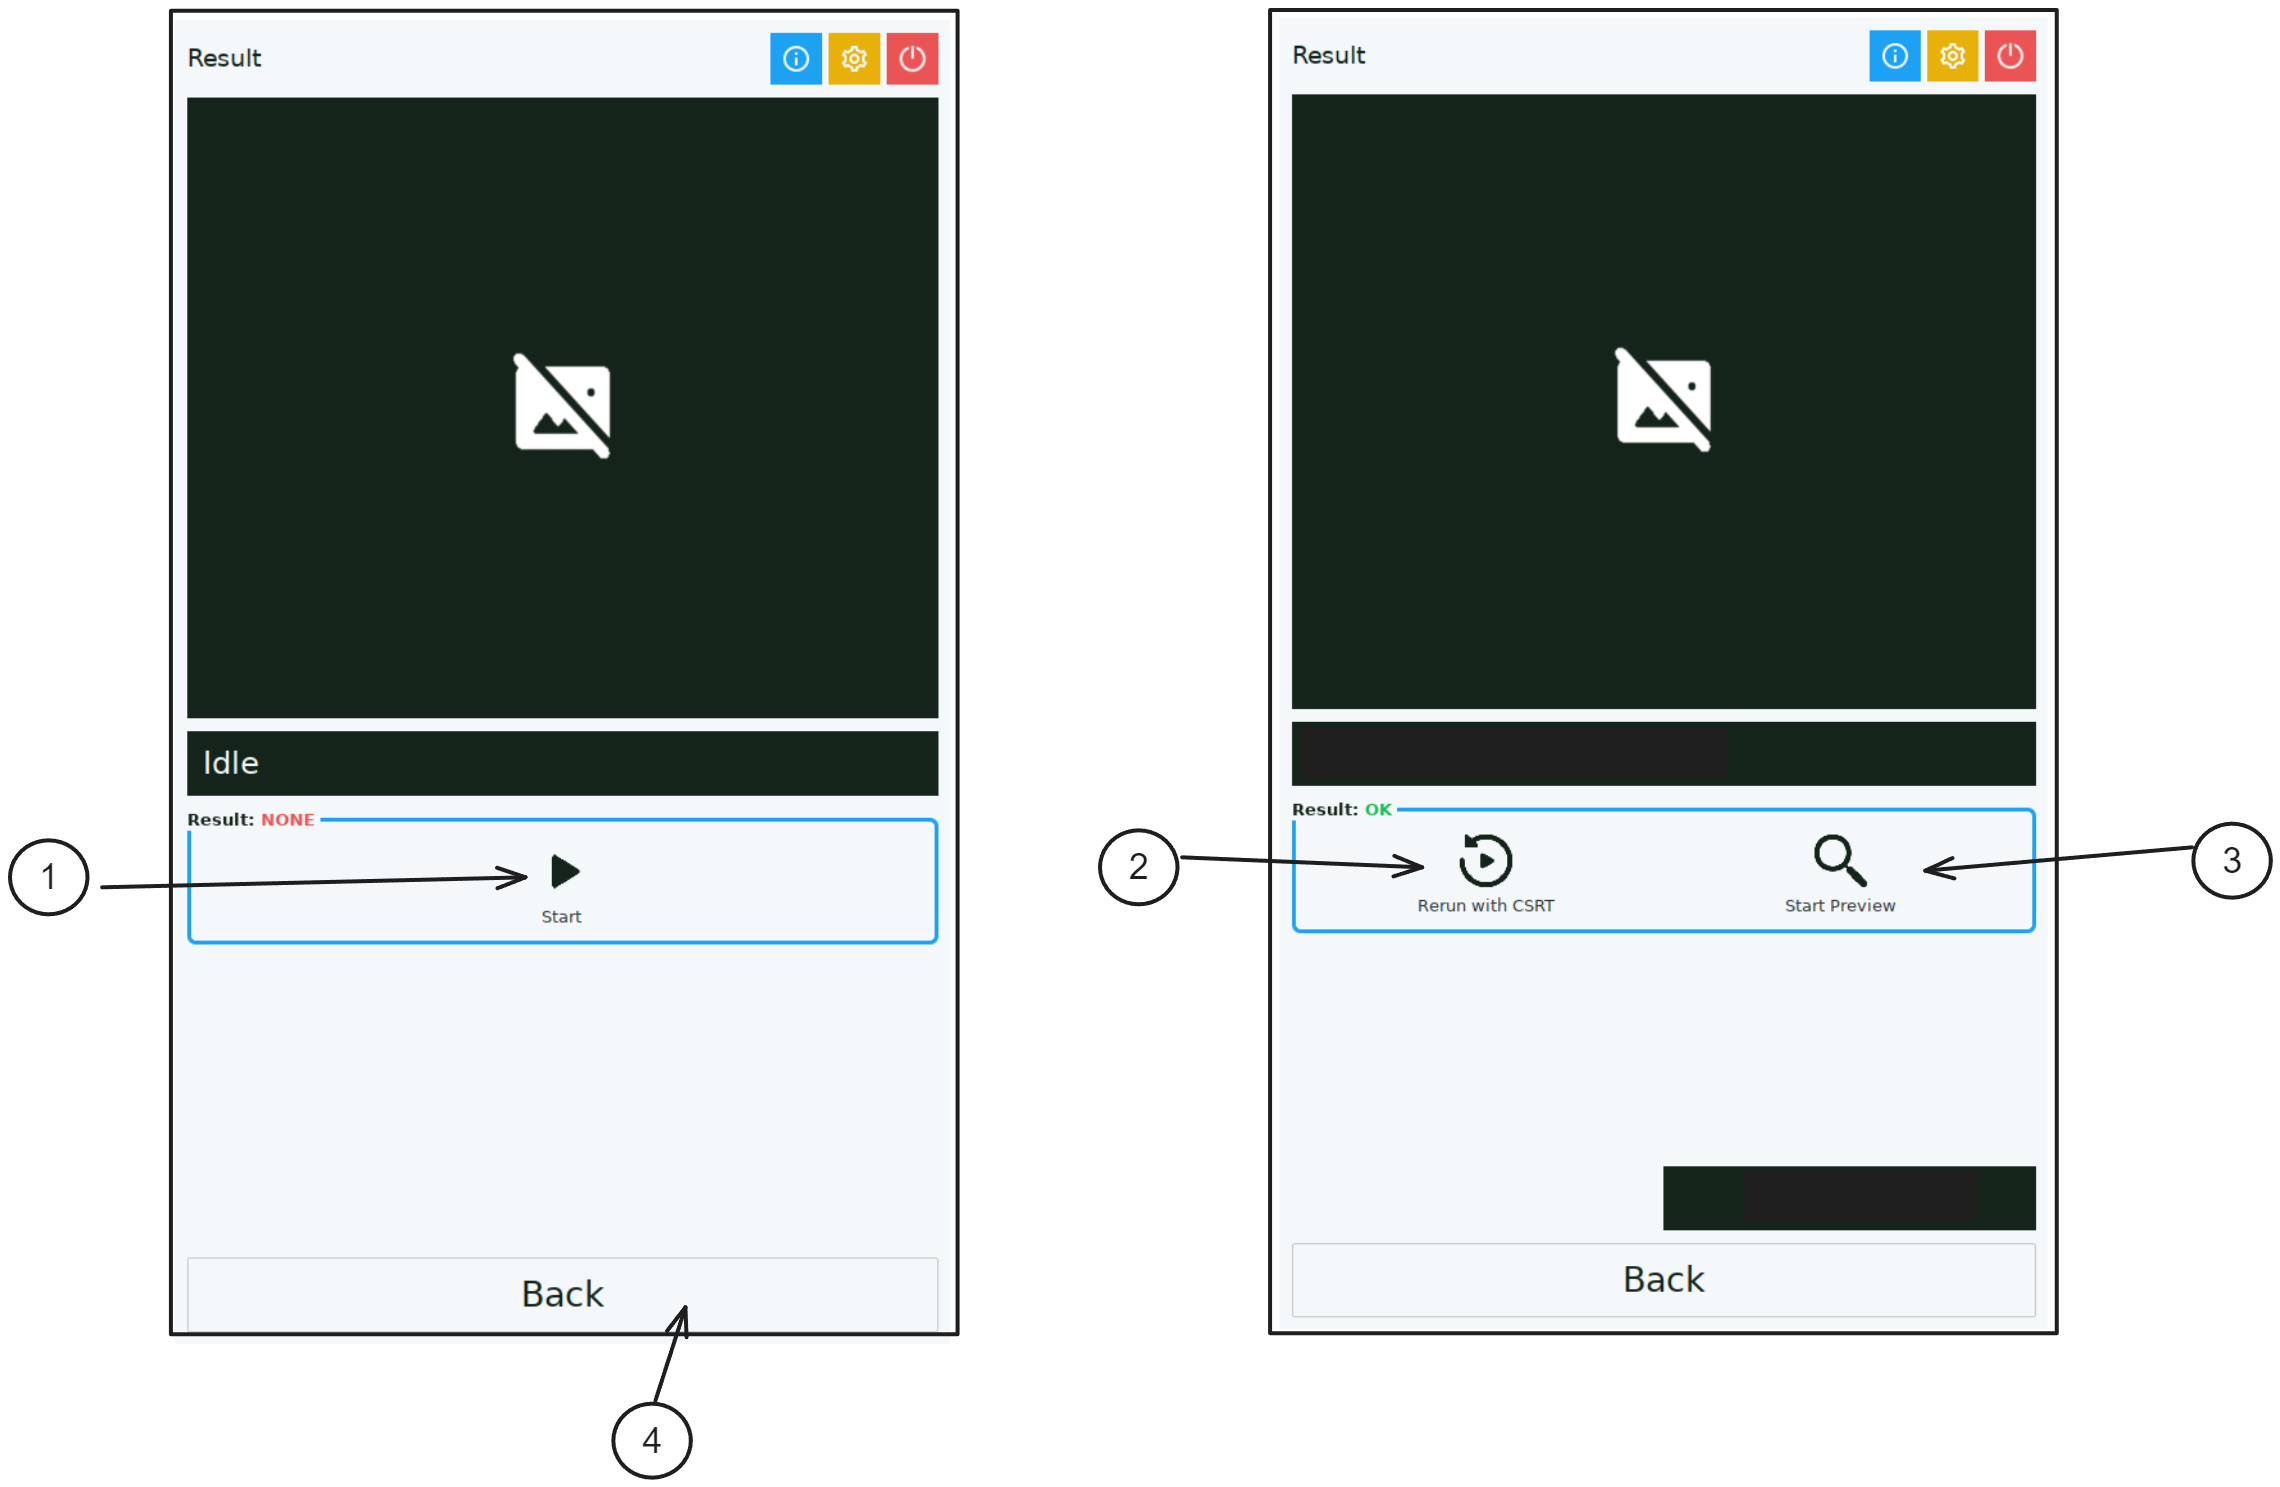
\includegraphics[width=\textwidth]{texs/chapter1/image/p5.png}
\end{figure}

\begin{table}[!ht]
    \centering
    \begin{tabular}{p{0.05\linewidth} | p{0.5\linewidth}}
        \hline
        \textbf{No.} & \textbf{Function}                            \\ \hline
        1            & Start Process Data with Optical Flow Tracker \\ \hline
        2            & Rerun Process With CSRT Tracker              \\ \hline
        3            & Preview Processed Data                       \\ \hline
        4            & Change To Capture Panel                      \\ \hline
    \end{tabular}
\end{table}

\subsection{Instructions}

\subsubsection{Start Process Data with Optical Flow Tracker}

The program is set to use the Optical Flow Tracker by default. To start processing the data, press the Process Data button (\textbf{1}). The program will start processing the data. The program will display the processed data in the panel.

\subsubsection{Rerun Process With CSRT Tracker}

In some cases, where the Optical Flow Tracker is not accurate, you can use the CSRT Tracker. To rerun the process with CSRT Tracker, press the Rerun Process button (\textbf{2}). The program will start processing the data with CSRT Tracker. The program will display the processed data in the panel.

\subsubsection{Preview Processed Data}

To preview the processed data press the Preview button (\textbf{3}). The program will display the processed data in the panel.

\subsubsection{Change To Capture Panel}

After processing the data, you can change to the Capture Panel by pressing the Back button (\textbf{4}). The Capture Panel will be displayed.

\pagebreak
\section{Color Calibration Panel}
\label{sec:color-calibration-panel}

The Color Calibration Panel is where you can perform color calibration. The purpose of this calibration is to detect the color of the mat, which is used within the \hyperref[sec:auto-lane-calibration-panel]{Automatic Lane Calibration Panel}.

\begin{figure}[H]
    \centering
    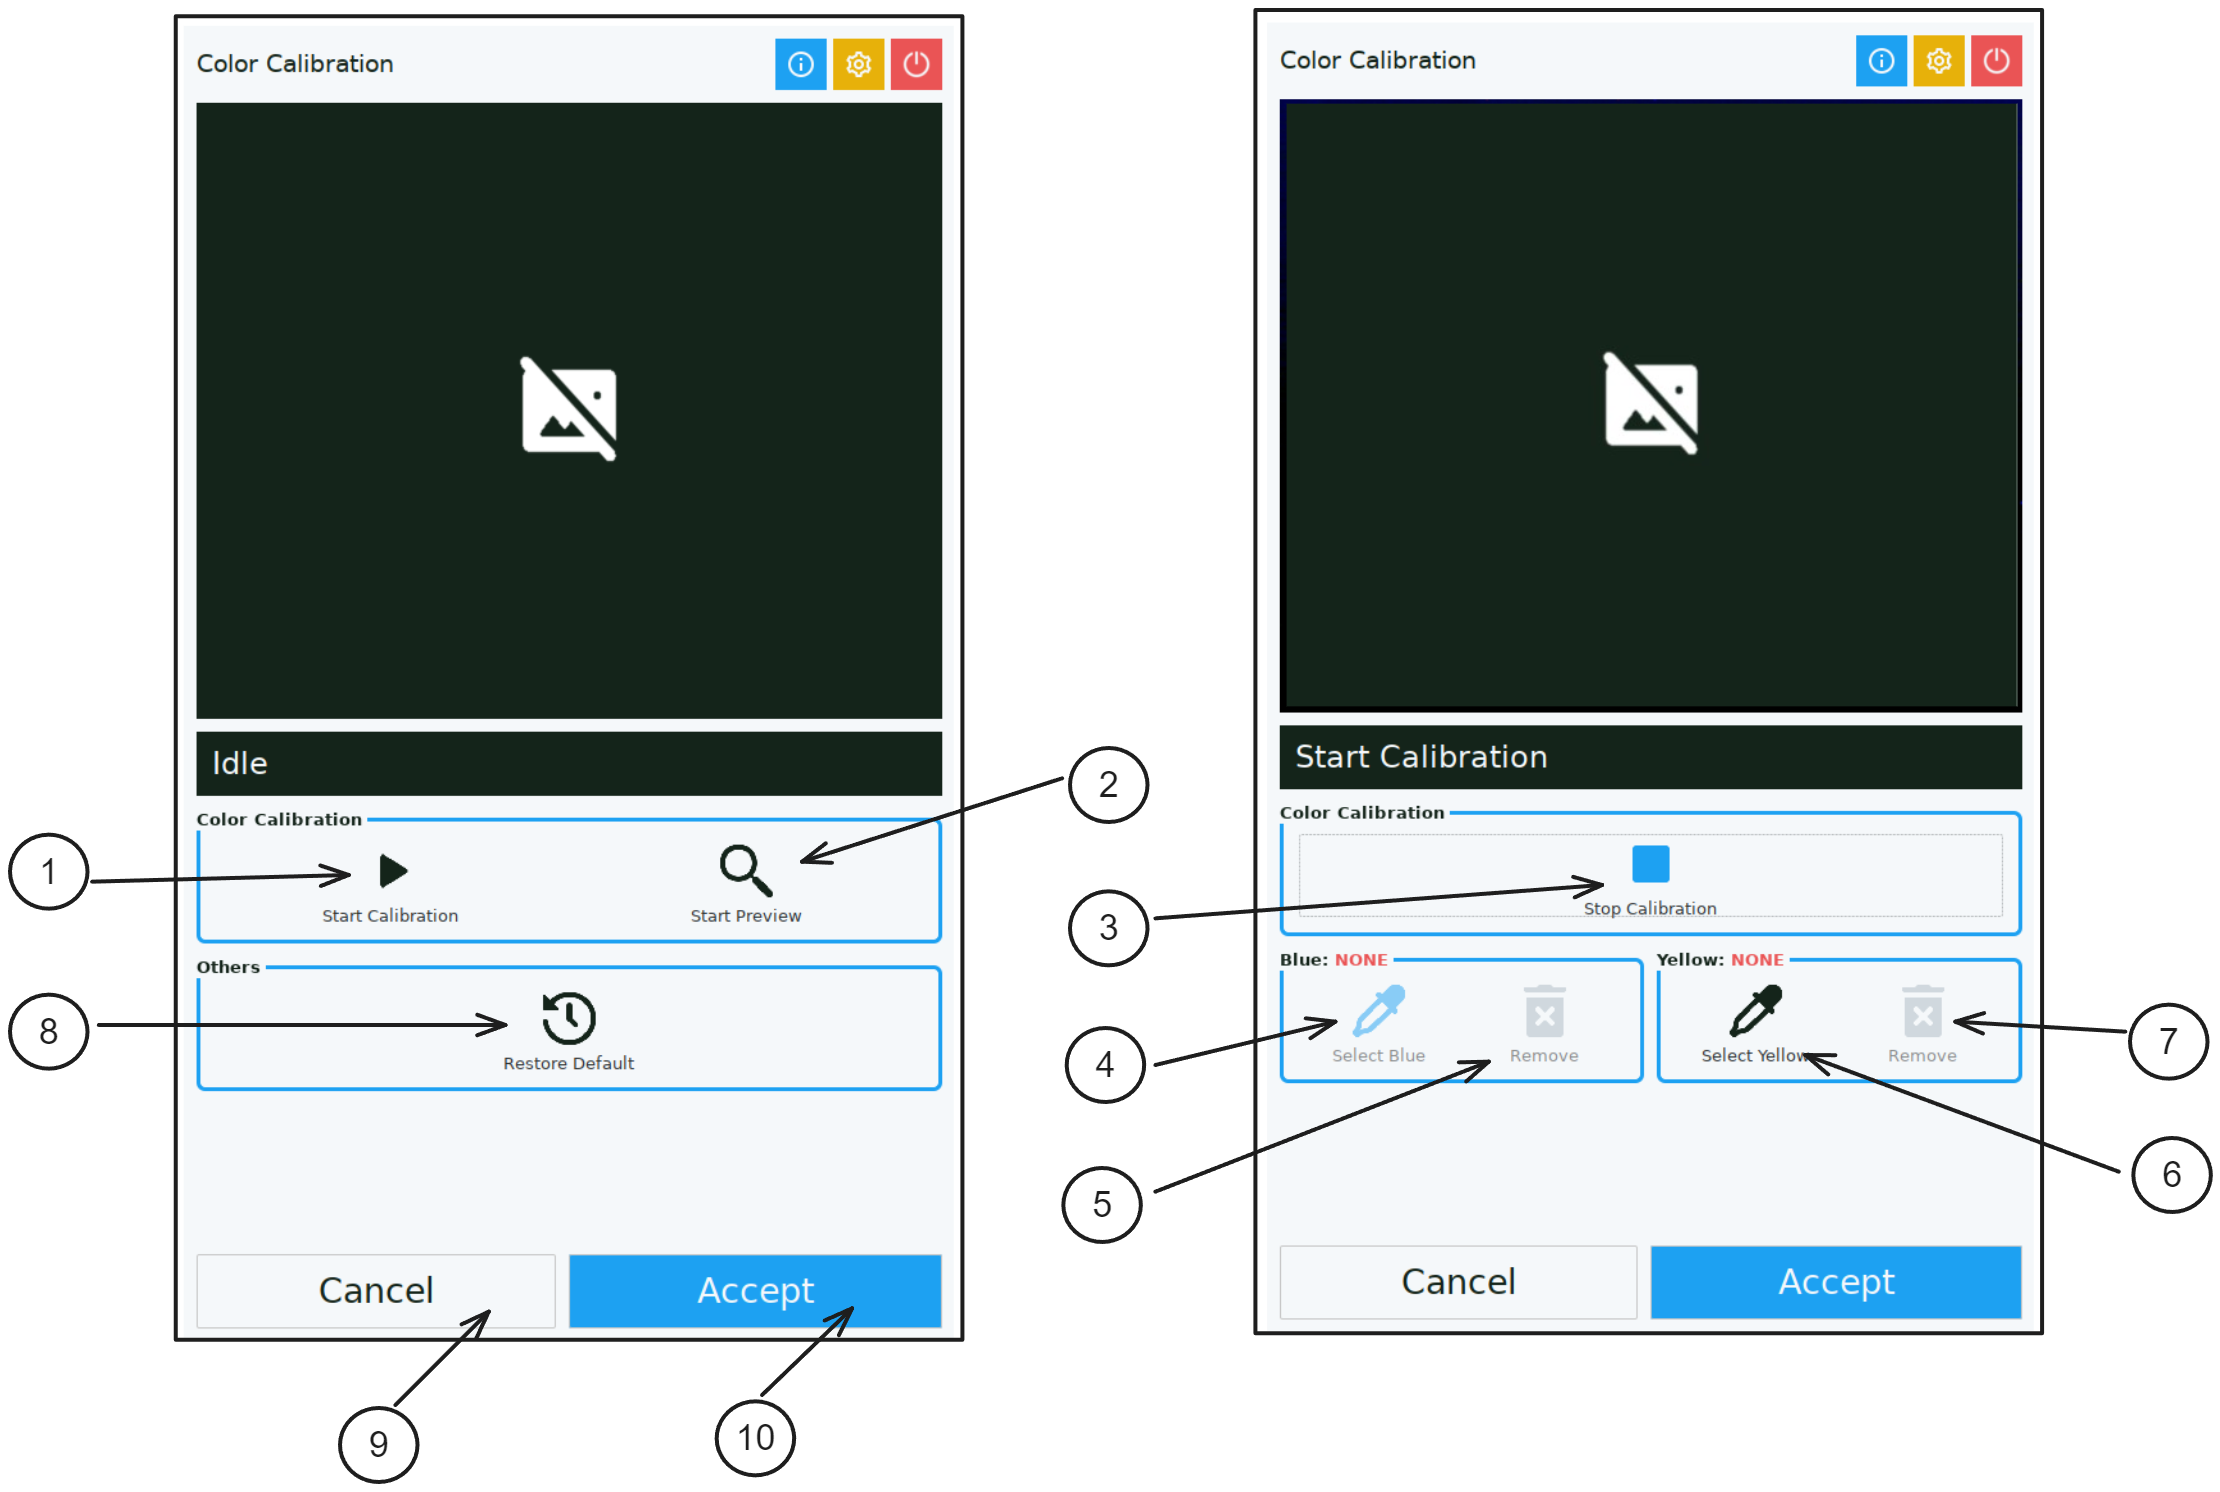
\includegraphics[width=\textwidth]{texs/chapter1/image/p6.png}
\end{figure}

\begin{table}[!ht]
    \centering
    \begin{tabular}{p{0.05\linewidth} | p{0.5\linewidth}}
        \hline
        \textbf{No.} & \textbf{Function}                \\ \hline
        1            & Start Color Calibration          \\ \hline
        2            & Preview Current Calibrated Color \\ \hline
        3            & Stop Calibration                 \\ \hline
        4            & Select Blue Color                \\ \hline
        5            & Remove Selected Blue Range       \\ \hline
        6            & Select Yellow Color              \\ \hline
        7            & Remove Selected Yellow Range     \\ \hline
        8            & Restore Default Range            \\ \hline
        9            & Cancel Calibration               \\ \hline
        10           & Accept Calibration               \\ \hline
    \end{tabular}
\end{table}


\subsection{Instructions}

\subsubsection{Performing Calibration}

To perform color calibration, press the Start Calibration button (\textbf{1}). The program will start the calibration process. The program will display the image in the panel. Begin with selecting the blue color by pressing the Select Blue Color button (\textbf{4}). Color selection is done via point and drag method. Place the finger on the Image Panel where the blue color is located The program will display the blue color range in the panel. If the range seems inaccurate, try to select another point. Repeat the process for the yellow color by pressing the Select Yellow Color button (\textbf{6}). After selecting both colors, press the Accept Calibration button (\textbf{10}). The program will save the calibration data in the program's memory.

\subsubsection{Preview Current Calibrated Color}

To preview the current calibrated color press the Preview button (\textbf{2}). The program will display the image in the panel. If the calibration data is present, the program will display the calibrated data in the panel.

\subsubsection{Restore Default Range}

To restore the default range press the Restore Default Range button (\textbf{8}). The program will restore the default range.


\pagebreak
\section{Trim Data Panel}
\label{sec:trim-data-panel}

The Trim Data Panel is where you can trim the captured data. In cases where the captured data is too long, you can trim the data to a certain length.\footnote{There is a limit to the minimum length of data (5 frames). Buttons will be disabled if the minimum length is reached.}\footnote{By performing the trim, the program will automatically remove the calibration data and ROI data. This is done to avoid any errors.}

\begin{figure}[H]
    \centering
    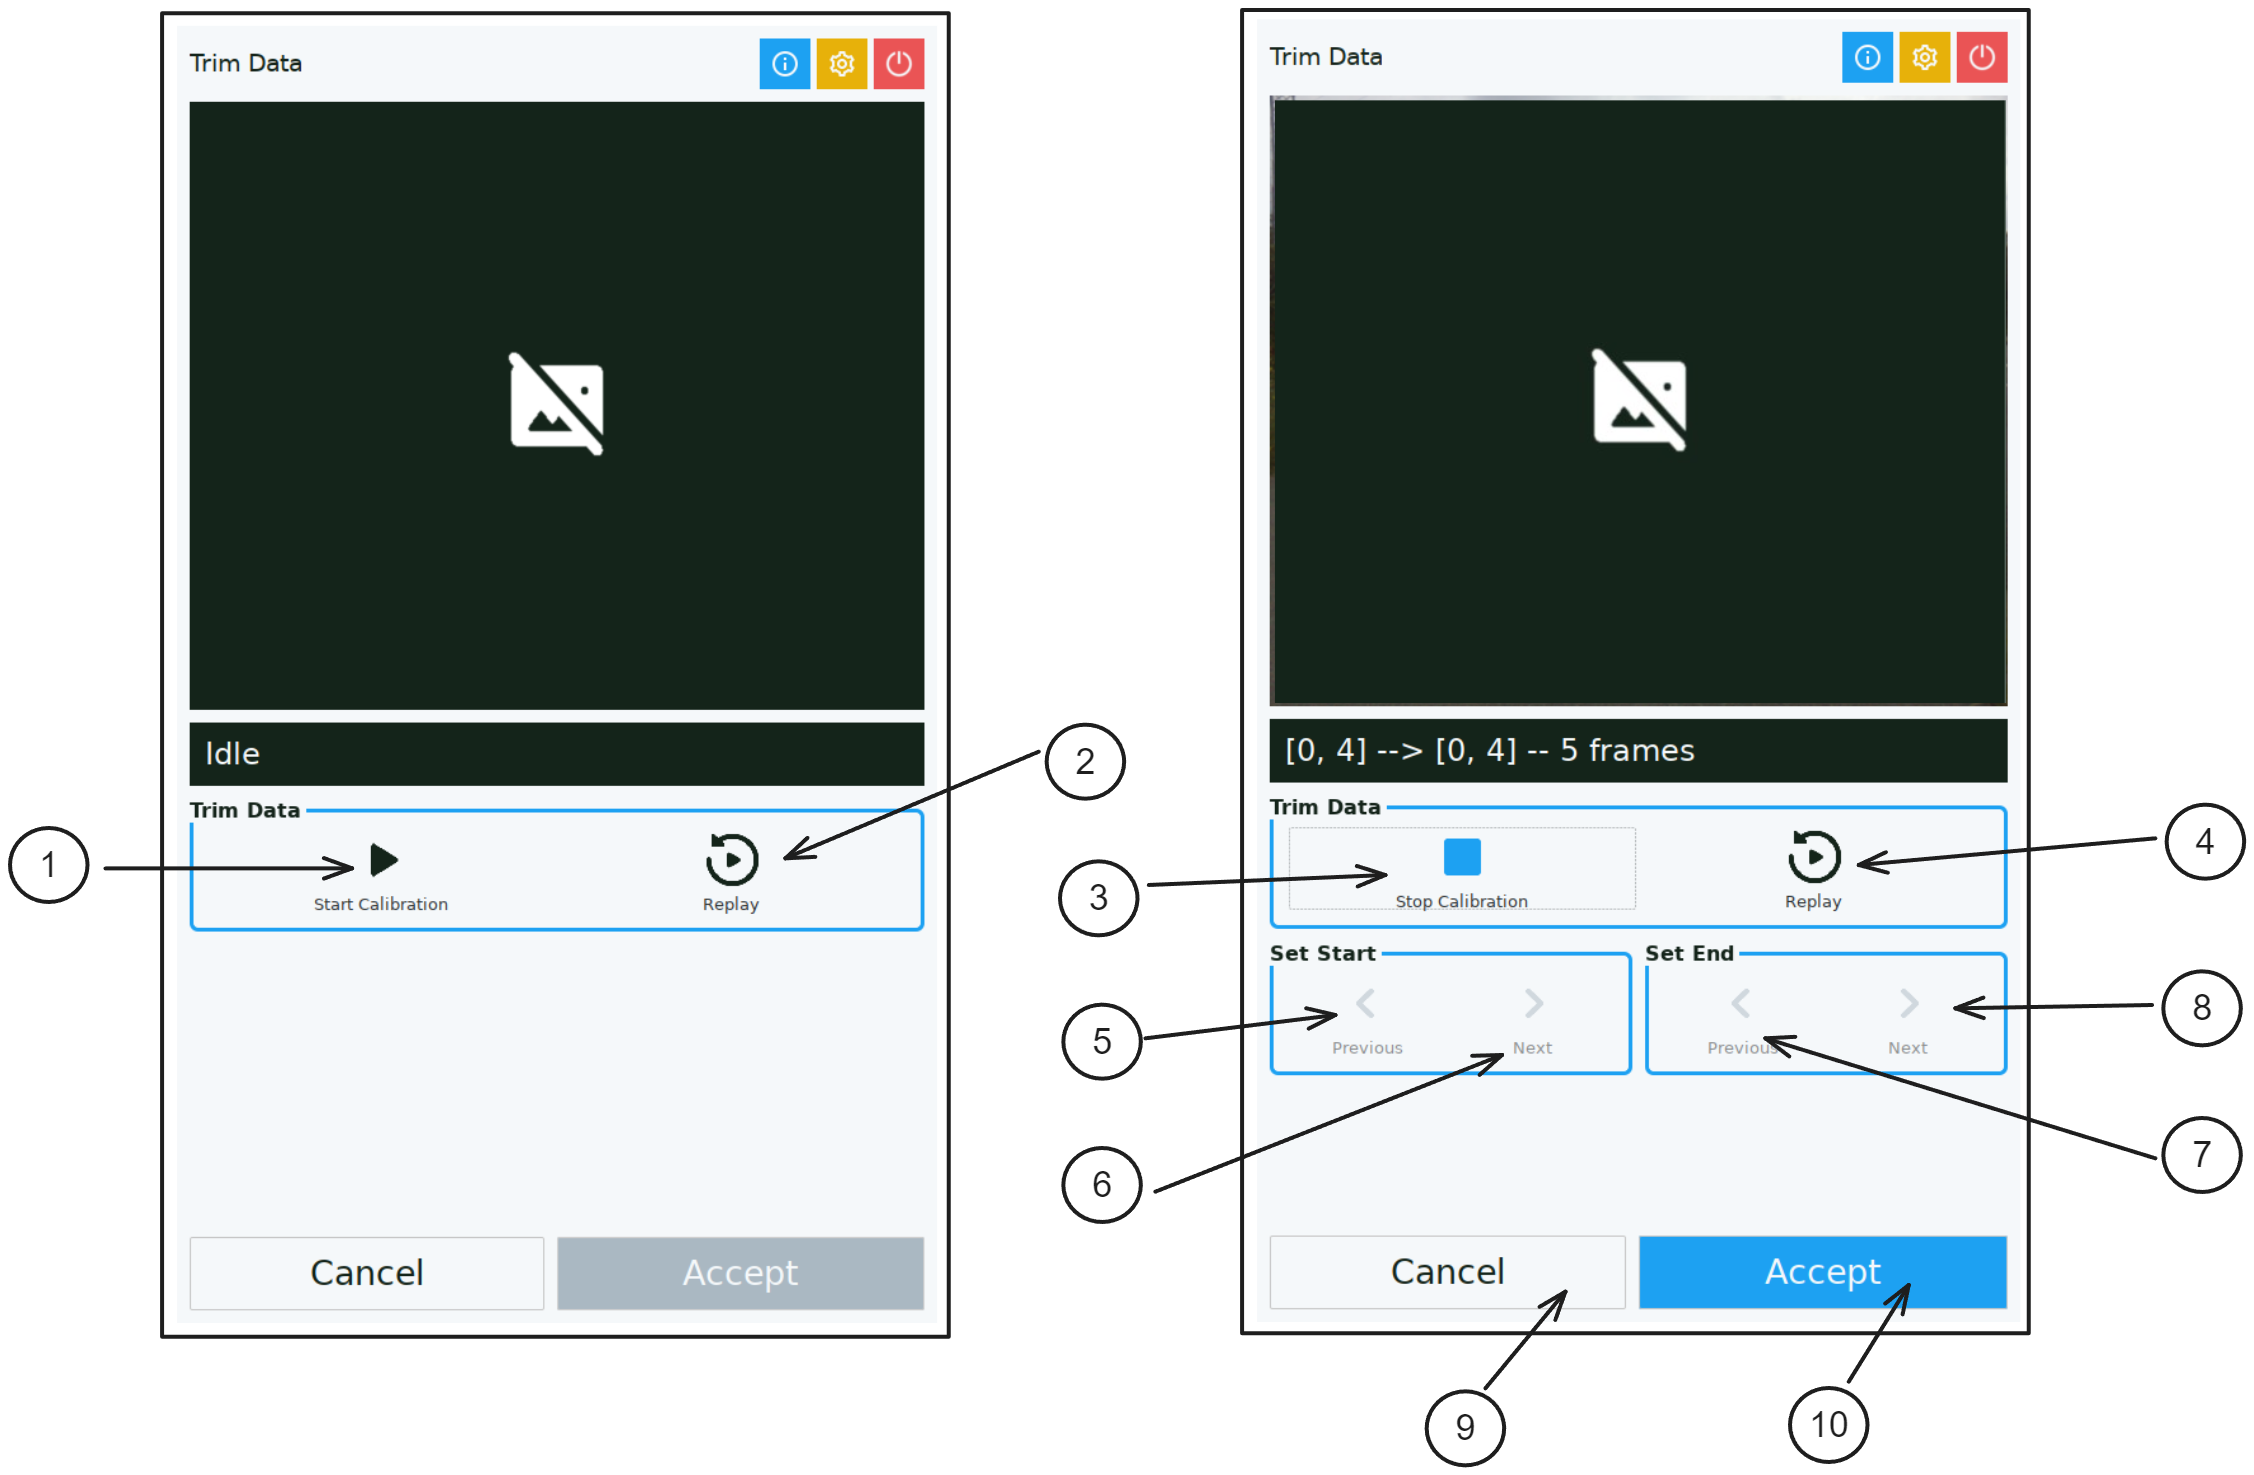
\includegraphics[width=\textwidth]{texs/chapter1/image/p7.png}
\end{figure}

\begin{table}[!ht]
    \centering
    \begin{tabular}{p{0.05\linewidth} | p{0.5\linewidth}}
        \hline
        \textbf{No.} & \textbf{Function}        \\ \hline
        1            & Start Trim Data          \\ \hline
        2            & Replay Current Data      \\ \hline
        3            & Stop Trim Data           \\ \hline
        4            & Replay Current Data      \\ \hline
        5            & Decrement Start Position \\ \hline
        6            & Increment Start Position \\ \hline
        7            & Decrement End Position   \\ \hline
        8            & Increment End Position   \\ \hline
        9            & Cancel                   \\ \hline
        10           & Accept                   \\ \hline
    \end{tabular}
\end{table}


\subsection{Instructions}

\subsubsection{Performing Trim}

To perform trim, press the Start Trim button (\textbf{1}). The program will start the trim process. The program will display the image in the panel. Begin with selecting the start position by pressing the Decrement Start Position button (\textbf{5}) or Increment Start Position button (\textbf{6}). The program will display the current start position in the panel. Repeat the process for the end position by pressing the Decrement End Position button (\textbf{7}) or Increment End Position button (\textbf{8}). After selecting both positions, press the Accept button (\textbf{10}). The program will save the trimmed data in the program's memory.

\subsubsection{Replay Current Data / Preview}

To replay the current data or preview the trimmed data press the Replay button (\textbf{2}). The program will replay the data in the panel.

\pagebreak
\section{Settings Panel}
\label{sec:settings-panel}

The Settings Panel is where you can adjust the settings of the application.

\subsection{Camera}

\subsubsection{Camera ID}
The Camera ID is the ID of the camera that will be used by the application. The default value is \textbf{0}. If you have multiple cameras, you can change the value to the ID of the camera you want to use.\footnote{\label{label1}Changing the value of this variable is disabled. However, the value can be manipulated directly by accessing the config file or through source code.}

\subsubsection{Camera Width}
The Camera Width is the width of the camera. The default value is \textbf{1280}. If you have a camera with a different width, you can change the value to the width of the camera.\cref{label1}

\subsubsection{Camera Height}
The Camera Height is the height of the camera. The default value is \textbf{960}. If you have a camera with a different height, you can change the value to the height of the camera.\cref{label1}

\subsubsection{Camera FPS}
The Camera FPS is the FPS of the camera. The default value is \textbf{10}. If you want to increase or decrease the FPS of the camera, you can change the value to the FPS of the camera.

\subsection{Sensor}

\subsubsection{Sensor Width}
The Sensor Width is the width of the sensor. The default value is \textbf{3.68} mm. If you have a sensor with a different width, you can change the value to the width of the sensor.\footnote{\label{label2}Variable is in mm.}

\subsubsection{Sensor Focal Length}
The Sensor Focal Length is the focal length of the sensor. The default value is \textbf{3.04} mm. If you have a sensor with a different focal length, you can change the value to the focal length of the sensor.\cref{label2}

\subsection{Capture}

\subsubsection{Max Frame}
The number of frames that will be captured. The default value is \textbf{10}. If you want to increase or decrease the number of frames, you can change the value to the number of frames.

\subsubsection{Debug - Show Image}
This variable is used to show image during capturing process. There seems to be a bug where when showing images during capturing will cause inaccuracy in timing of the capturing process. The default value is \textbf{false}. If you want to show the image during capturing process, you can change the value to true.

\subsubsection{Debug - Save Data}
This variable is used to save data during capturing process. The default value is \textbf{false}. If the variable is enabled, the data will always be automatically saved for each capturing process.

\subsection{Model}

\subsubsection{Maximum Thread Pool}
The maximum number of threads that will be used by the application. The default value is \textbf{2}. If you want to increase or decrease the number of threads, you can change the value to the number of threads.

\subsection{Optical Flow}

Refer to OpenCV documentation for more information.

\subsubsection{Max Corners}
The maximum number of corners that will be detected by the Optical Flow Tracker. The default value is \textbf{1000}. If you want to increase or decrease the number of corners, you can change the value to the number of corners.

\subsubsection{Quality Level}
The quality level of the corners that will be detected by the Optical Flow Tracker. The default value is \textbf{0.05}. If you want to increase or decrease the quality level, you can change the value to the quality level.

\subsubsection{Minimum Distance}
The minimum distance between corners that will be detected by the Optical Flow Tracker. The default value is \textbf{7}. If you want to increase or decrease the minimum distance, you can change the value to the minimum distance.

\subsubsection{Block Size}
The block size of the corners that will be detected by the Optical Flow Tracker. The default value is \textbf{3}. If you want to increase or decrease the block size, you can change the value to the block size.

\subsubsection{Use Harris Detector}
This variable is used to enable or disable the Harris Detector. The default value is \textbf{false}. If you want to enable the Harris Detector, you can change the value to true.

\subsubsection{K}
The K value of the Harris Detector. The default value is \textbf{0.04}. If you want to increase or decrease the K value, you can change the value to the K value.

\subsubsection{Minimum Point Distance}
The minimum distance between points that will be detected by the Optical Flow Tracker. Any value below this value will be ignored. The default value is \textbf{0.2}. If you want to increase or decrease the minimum distance, you can change the value to the minimum distance.

\subsubsection{Threshold}
The minimum distance between points that will be detected by the Optical Flow Tracker. Any value below this value will be ignored. The default value is \textbf{0.2}. If you want to increase or decrease the minimum distance, you can change the value to the minimum distance.

\subsection{Measurement}

\subsubsection{Object Width}
The width of the object that will be used for measurement. The default value is \textbf{3500} mm. If you have an object with a different width, you can change the value to the width of the object.\footnote{This variable is used together with the \textbf{DISTANCE MEASUREMENT MODE}. Refer to \hyperref[sec:auto-lane-calibration-panel]{Automatic Lane Calibration Panel} and \hyperref[sec:manual-lane-calibration-panel]{Manual Lane Calibration Panel} for more information.}

\subsubsection{Object Height}
The height of the object that will be used for measurement. The default value is \textbf{2000} mm. If you have an object with a different height, you can change the value to the height of the object.\footnote{This variable is used together with the \textbf{DISTANCE MEASUREMENT MODE}. Refer to \hyperref[sec:distance-calibration-panel]{Distance Calibration Panel} for more information.}

\subsection{Preview}

\subsubsection{Preview Width}
The width of the preview image. The default value is \textbf{640}. If you want to increase or decrease the width of the preview image, you can change the value to the width of the preview image.\footnote{\label{label3}This variable is used to display image within Image Panel. Lowering the value will increase the performance of the application.}

\subsubsection{Preview Height}
The height of the preview image. The default value is \textbf{480}. If you want to increase or decrease the height of the preview image, you can change the value to the height of the preview image.\cref{label3}

\subsection{RANSAC}

\subsubsection{Threshold}
The minimum distance to consider a point as an inlier. The default value is \textbf{6.0}. If you want to increase or decrease the threshold, you can change the value to the threshold.

\subsubsection{Minimum Point}
The minimum number of data within the datasets to enable line searching. Default value is \textbf{50}. If you want to increase or decrease the minimum point, you can change the value to the minimum point.

\subsubsection{Maximum Iteration}
The maximum number of iteration to find the best line. Default value is \textbf{500}. If you want to increase or decrease the maximum iteration, you can change the value to the maximum iteration.

\subsection{Blue HSV}

\subsubsection{Hue}
The hue value of the blue color. The default value is \textbf{130} for Upper and \textbf{100} for Lower.

\subsubsection{Saturation}
The saturation value of the blue color. The default value is \textbf{255} for Upper and \textbf{100} for Lower.

\subsubsection{Value}
The value of the blue color. The default value is \textbf{255} for Upper and \textbf{100} for Lower.

\subsection{Yellow HSV}

\subsubsection{Hue}
The hue value of the yellow color. The default value is \textbf{35} for Upper and \textbf{20} for Lower.

\subsubsection{Saturation}
The saturation value of the yellow color. The default value is \textbf{255} for Upper and \textbf{100} for Lower.

\subsubsection{Value}
The value of the yellow color. The default value is \textbf{255} for Upper and \textbf{100} for Lower.

\subsection{Threads}

Variable to enable automatic process starting when switching panel.

\subsubsection{Auto Calibration}
This variable is used to enable or disable automatic calibration when switching to the Calibration Panel. The default value is \textbf{false}. If you want to enable automatic calibration, you can change the value to true.\footnote{This variable is unused.}

\subsubsection{Auto Manual Calibration}
When enabled, the program will automatically start manual calibration when switching to the Manual Lane Calibration Panel. The default value is \textbf{false}. If you want to enable automatic manual calibration, you can change the value to true.

\subsubsection{Auto ROI}
When enabled, the program will automatically start ROI selection when switching to the ROI Panel. The default value is \textbf{false}. If you want to enable automatic ROI selection, you can change the value to true.

\subsubsection{Auto Result}
When enabled, the program will automatically start processing data when switching to the Result Panel. The default value is \textbf{false}. If you want to enable automatic processing data, you can change the value to true.
